%% Journal of Glaciology submission template.
%% Primary structural guide: IGS class demo (igs2eannalsguide.tex in the AOG zip).
%% Secondary section-organisation guide: Fisser et al. (2024) (papers/Fisser2024.pdf).
%% Authoritative project state: ../../plan.md + ../../reference/*.md + ../../iceberg-rework-README.md.
%%
%% Options:
%%   "review" = single-column submission layout. Remove to preview two-column JGlac output.
%%   "jog"    = Journal of Glaciology. Use "aog" for Annals of Glaciology.
\documentclass[review,jog]{igs}

\usepackage[utf8]{inputenc}
\usepackage{mathabx}
\usepackage{graphicx}
\usepackage{siunitx}
\usepackage{booktabs}

% Journal metadata (left blank until acceptance; JGlac production fills these).
\jourvolume{}
\jourissue{}
\jourpubyear{2026}

\begin{document}

% TODO: finalise title and running-head short title.
\title[Short running-head title]{Full paper title placeholder}

% TODO: author list. IGS house style uses CAPS for surnames.
% Keep affiliation superscripts matching \affiliation{} below.
\author[First and others]{First AUTHOR,$^1$
  Second AUTHOR,$^1$
  Third AUTHOR$^2$}

\affiliation{%
$^1$[Department], Bowdoin College, Brunswick, ME, USA\\
$^2$[Collaborator affiliation]\\
  Correspondence: [Corresponding author name] \email{[email]}}

\begin{frontmatter}

\maketitle

\begin{abstract}
Small icebergs are a primary control on submarine-melt freshwater fluxes in Greenland fjords, but standard near-infrared (NIR) threshold detection on Sentinel-2 imagery breaks down at solar zenith angles (SZA) above 65$^\circ$ where shadowed iceberg faces fall below threshold and ocean reflectance rises. We train a UNet++ segmentation model with a ResNet34 encoder on 916 Sentinel-2 chips spanning SZA $<$ 65$^\circ$ to $>$ 75$^\circ$ in Kangerlussuaq and Sermilik fjords, east Greenland, and compare six area-retrieval methods: a fixed B08 threshold, per-chip Otsu, UNet++ argmax, and three UNet++ post-processing variants (threshold on probabilities, Otsu on probabilities, and dense conditional random field). Per-pair Hungarian matching with $\mathrm{IoU} \geq 0.30$ yields a Fisser-comparable mean absolute error in iceberg root length and a per-pair IoU on matched pairs. UNet++ + DenseCRF achieves the lowest per-pair root-length error in three of four SZA bins (12.6 m at SZA $>$ 75$^\circ$ vs.\ 20.1 m for the fixed threshold); UNet++ + Otsu wins lt65. A controlled preprocessing isolation shows that the 40 m component filter and annotation-aware ice-coverage pixel mask, while consistent with prior work, degrade model calibration in low-data regimes and should be reported as a controlled variable rather than a fixed pipeline choice.
\end{abstract}

\end{frontmatter}


%% =======================================================================
%% Section organisation follows Fisser (2024) / JGlac Article convention:
%%   1. Introduction
%%   2. Study area and data
%%   3. Methods
%%   4. Results
%%   5. Discussion
%%   6. Conclusion
%%   + Acknowledgements, References, (Appendices)
%% IGS default is unnumbered sections (secnumdepth=0). Uncomment below to number.
%% \setcounter{secnumdepth}{2}
%% =======================================================================


\section{Introduction}

Iceberg calving is a major component of Greenland Ice Sheet mass loss \citep{Enderlin2014, Alley2023}. Accurate iceberg area inventories are required to estimate submarine melt-driven freshwater fluxes into fjord systems \citep{Moon2018, Rezvanbehbahani2020} and to parameterise iceberg drift and deterioration models used in maritime hazard forecasting \citep{Keghouche2010, Marchenko2019}. Satellite optical imagery, in particular the Sentinel-2 near-infrared band (B08) at 10 m resolution, is the primary tool for retrieving above-waterline iceberg areas in Greenland fjords \citep{Sulak2017, Scheick2019}. Icebergs smaller than 100 m in root length contribute disproportionately to the total freshwater budget but are systematically underrepresented in existing inventories because they fall near or below the detection limits of per-pixel methods \citep{Rezvanbehbahani2020}. Extending reliable retrieval across all iceberg size classes and across the full range of seasonal illumination conditions is therefore necessary for closing regional calving budgets \citep{Moyer2019}.

The standard approach to optical iceberg detection applies a fixed reflectance threshold to B08, classifying pixels above a calibrated cutoff as ice \citep{Sulak2017, Moyer2019, Scheick2019}. \citet{Fisser2024} calibrated a threshold of B08 $\geq$ 0.12 against airborne reference data at SZA 56$^\circ$ and evaluated its stability across 14 Kangerlussuaq acquisitions spanning SZA 45$^\circ$ to 81$^\circ$. Below SZA 65$^\circ$, standardised area error remained within $+5.9$ \% to $-5.7$ \%; above 65$^\circ$, error grew and became inconsistent. Two physical mechanisms drive this degradation. At high SZA, iceberg surfaces segregate into sun-facing slopes and shadowed faces, causing shadow pixels to fall below the threshold and producing systematic area underestimation \citep{Fisser2024, Gardner2010}. Simultaneously, ocean NIR reflectance rises, compressing the spectral contrast between ice and water and inflating false-positive rates \citep{Pegau2001}. \citet{Fisser2024} characterised these errors under manually curated conditions: cloud cover below 2 \%, sea-ice concentration below approximately 10 \%, and only icebergs with root length above 100 m. The European Space Agency recommends a SZA limit of 70$^\circ$ for Sentinel-2 acquisitions \citep{ESA2019}. What is needed, but does not yet exist, is a retrieval approach that remains robust to the dual failure modes of shadowing and ocean brightening at SZA well above 65$^\circ$, that operates under automated rather than manually curated processing conditions, and that does not exclude the small-iceberg population from its detection scope.

Convolutional neural networks encode spatial relationships between neighbouring pixels, offering a mechanism for distinguishing shadowed ice from open water that per-pixel thresholds lack. Encoder-decoder architectures have demonstrated strong segmentation performance in cryosphere remote sensing, including iceberg delineation in Greenland fjords \citep{Rezvanbehbahani2020} and calving front extraction from SAR imagery \citep{Baumhoer2019}. This study trains a binary UNet++ model \citep{Zhou2018} with a ResNet34 encoder \citep{He2016} on 916 labelled Sentinel-2 chips spanning SZA $<$ 65$^\circ$ to $>$ 75$^\circ$ in Kangerlussuaq and Sermilik fjords, east Greenland. Annotations combine 398 chips from \citet{Fisser2024} at SZA $<$ 65$^\circ$ with 586 chips annotated for this work at SZA $\geq$ 65$^\circ$ using a SAM3 smart-select tool followed by manual review. Shadow pixels (Fisser class 2) are merged into iceberg before training, and connected components below 16 pixels (40 m root length) are removed from both annotation sources. The binary segmentation model is paired with five additional area-retrieval methods for comparison: a fixed B08 threshold, per-chip Otsu, UNet++ argmax, UNet++ + threshold on probabilities, UNet++ + Otsu on probabilities, and UNet++ + dense conditional random field. All six methods are evaluated by Hungarian per-pair matching with $\mathrm{IoU} \geq 0.30$, producing both Fisser-comparable mean absolute errors on iceberg root length and per-pair IoU on matched pairs, stratified into four SZA bins. Three questions structure the analysis:

\begin{enumerate}
\item To what extent does UNet++ segmentation, which incorporates learned spatial context, reduce the SZA-dependent area bias that fixed and adaptive NIR thresholding exhibits above 65$^\circ$?
\item At extreme SZA ($>$ 70$^\circ$, beyond ESA's recommended acquisition limit), how does the variance and magnitude of UNet++ area retrieval compare to threshold baselines across two independent fjord systems?
\item Among adaptive thresholding, dense conditional random field post-processing, and white top-hat morphological recovery, which post-processing rules give the most reliable segmentation and small-iceberg recovery without changing the model architecture?
\end{enumerate}

This paper demonstrates that learned segmentation maintains area retrieval consistency at solar zenith angles where threshold methods produce order-of-magnitude overestimates, and that conditional random field post-processing on UNet++ probabilities further reduces per-pair error in three of four SZA bins. Section 2 describes the study design, imagery, annotation sources, and detection methods. Section 3 presents area retrieval results stratified by SZA bin, including a controlled isolation of the preprocessing pipeline as a single experimental variable. Section 4 discusses the implications for extending automated iceberg monitoring into the low-illumination season.


\section{Study area and data}

\subsection{Study regions and imagery}

The study uses Sentinel-2 Level-1C imagery from two east Greenland fjord systems: Kangerlussuaq (KQ, $\sim$ 68.5$^\circ$ N) and Sermilik (SK, $\sim$ 65.7$^\circ$ N). Both fjords drain marine-terminating outlet glaciers of the Greenland Ice Sheet and contain iceberg populations that vary in size, density, illumination, and background complexity. Imagery is represented as 256 $\times$ 256 pixel chips, corresponding to 2.56 $\times$ 2.56 km at the Sentinel-2 10 m grid.

Each chip contains three top-of-atmosphere reflectance bands: B04 (red, 665 nm), B03 (green, 560 nm), and B08 (near-infrared, 842 nm). The UNet++ model receives all three bands. The threshold baselines use B08 because that is the band used in the Fisser threshold workflow and because near-infrared reflectance provides the strongest simple contrast between iceberg ice and dark water.

Scenes are grouped by solar zenith angle (SZA) into four bins: SZA $<$ 65$^\circ$, 65--70$^\circ$, 70--75$^\circ$, and $>$ 75$^\circ$. These bins follow the previous finding that threshold-based area retrieval begins to degrade near SZA 65$^\circ$ \citep{Fisser2024}. The binning also keeps the visual story simple: low-SZA scenes provide the Fisser-like anchor, while the higher bins test increasingly difficult autumn illumination conditions.

\subsection{Radiometric convention}

All threshold values in this paper are reported in the uncorrected reflectance convention used by the working pipeline. Sentinel-2 processing baselines N0500 and later distribute band digital numbers with a $+1000$ offset. The local chip pipeline scales digital numbers by $10^{-4}$ but does not subtract that offset. As a result, reflectance values are shifted upward by 0.10 relative to the corrected convention used by \citet{Fisser2024}. \citet{Fisser2024} used B08 $\geq$ 0.12; in this pipeline the equivalent fixed threshold is B08 $\geq$ 0.22. Because all chips are processed under the same convention, this offset does not affect within-study method comparisons.

\subsection{Chip filtering}

\begin{figure}[h]
\centering
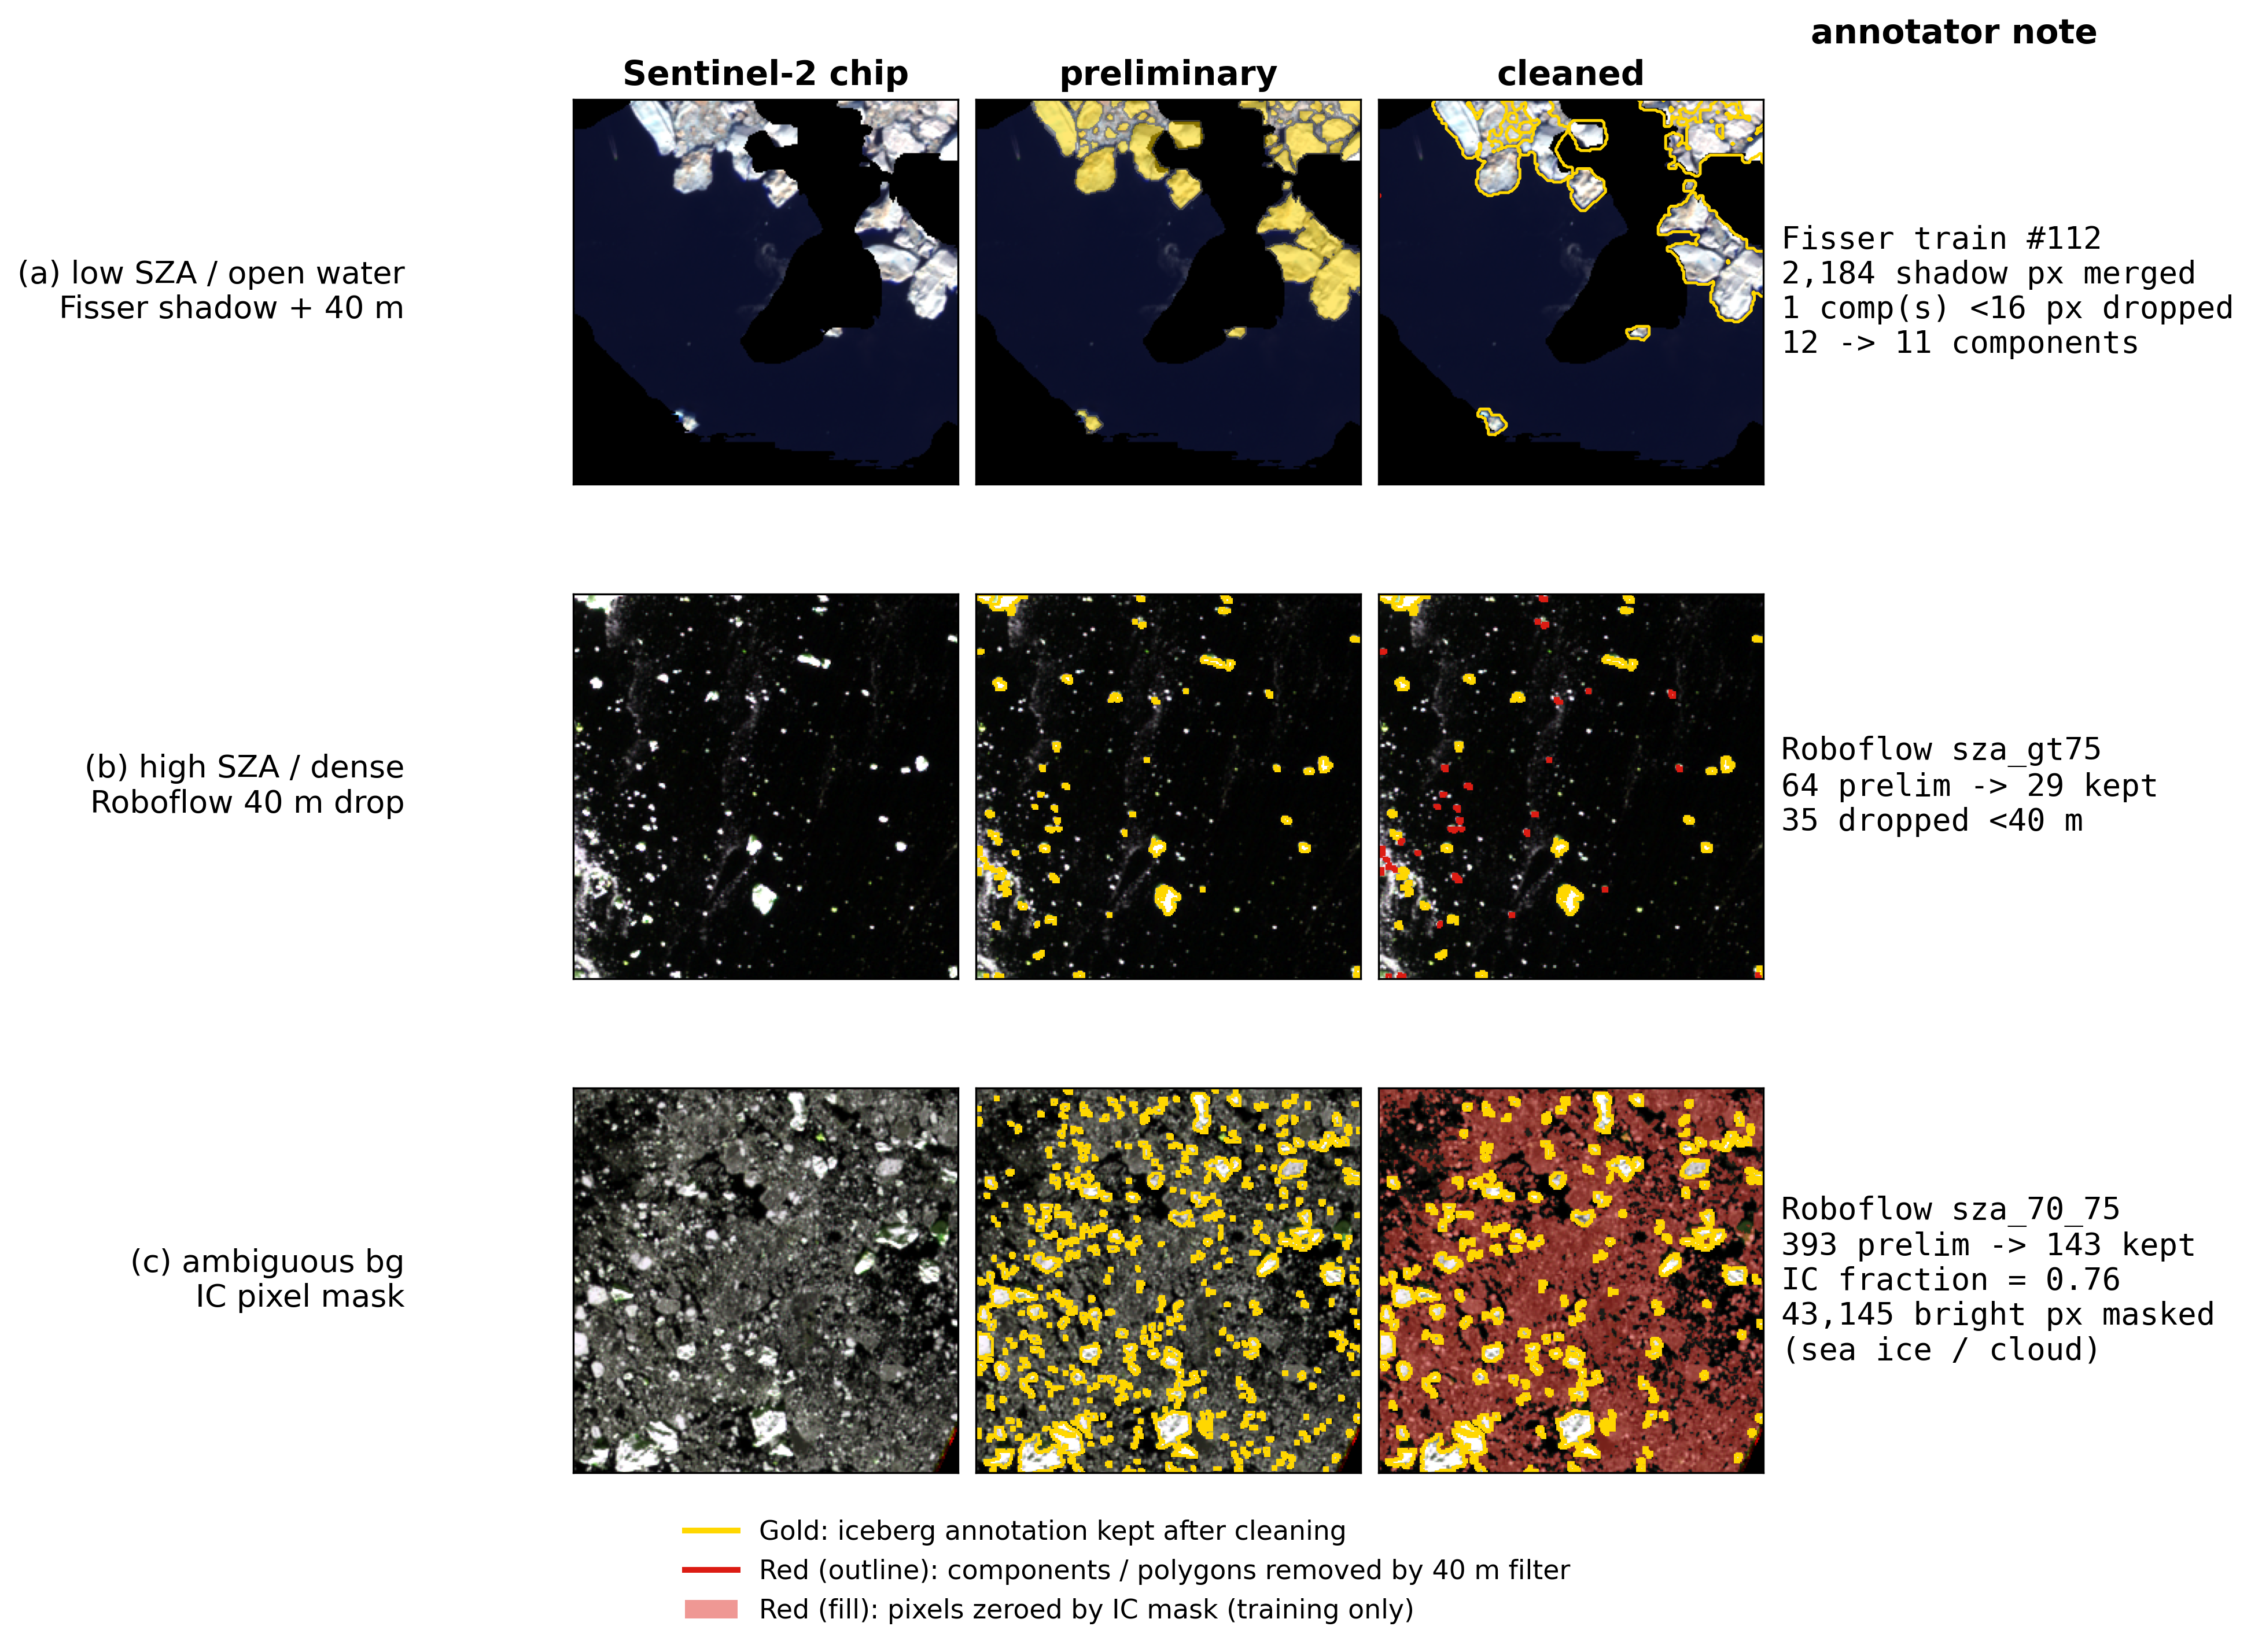
\includegraphics[width=\linewidth]{figures/fig-archive/20260501_202440__fig01_annotation_difficulty.png}
\caption{\textbf{Fig. 1.} Annotation-cleaning operations on three representative Sentinel-2 chips. Columns: false-color chip; preliminary annotation (gold iceberg, grey shadow); cleaned annotation; annotator note. In the cleaned column, gold marks iceberg annotations kept after cleaning, red outlines mark components or polygons removed by the 40 m filter, and the red translucent fill marks pixels zeroed by the training-time IC mask. (a) Low-SZA Fisser chip (fisser\_0112): 2{,}184 shadow pixels merged into iceberg, one sub-16 px component dropped (12 $\rightarrow$ 11 components; max iceberg root length 601 m, median 133 m). (b) High-SZA Roboflow chip: 35 of 64 polygons removed by the 40 m filter, leaving 29. (c) Mixed-background chip with IC fraction 0.76: IC pixel mask zeros 43{,}145 bright non-annotated pixels in training; the 143 kept iceberg annotations stay outlined in gold. Validation and test chips are never masked.}
\label{fig:fig01_annotation_difficulty}
\end{figure}

Individual connected components smaller than 16 pixels are removed from the binary masks. At 10 m resolution this corresponds to 1{,}600 m$^2$, or a square-root area of 40 m. The filter removes rasterisation fragments and sub-resolution speckle while retaining the smallest icebergs that can be consistently delineated in Sentinel-2 imagery. This cutoff is applied before the dataset split and is therefore part of the dataset definition rather than a post-hoc evaluation filter.

The pipeline also adapts the Fisser ice-coverage screen to chip-scale training data. Ice coverage (IC) is computed as the fraction of non-annotated pixels with B08 $\geq$ 0.22. If a training chip exceeds 15 \% by this annotation-aware calculation, bright non-annotated pixels are masked to zero across all three bands. Annotated iceberg pixels are preserved. Validation and test chips are never masked, so final metrics are measured on realistic, unmodified imagery. Across v4\_clean, 193 of 551 training chips meet the masking criterion (5.9 million non-iceberg pixels zeroed; 1.4 million annotated iceberg pixels retained).

\subsection{Annotation sources and dataset composition}

\begin{figure}[h]
\centering
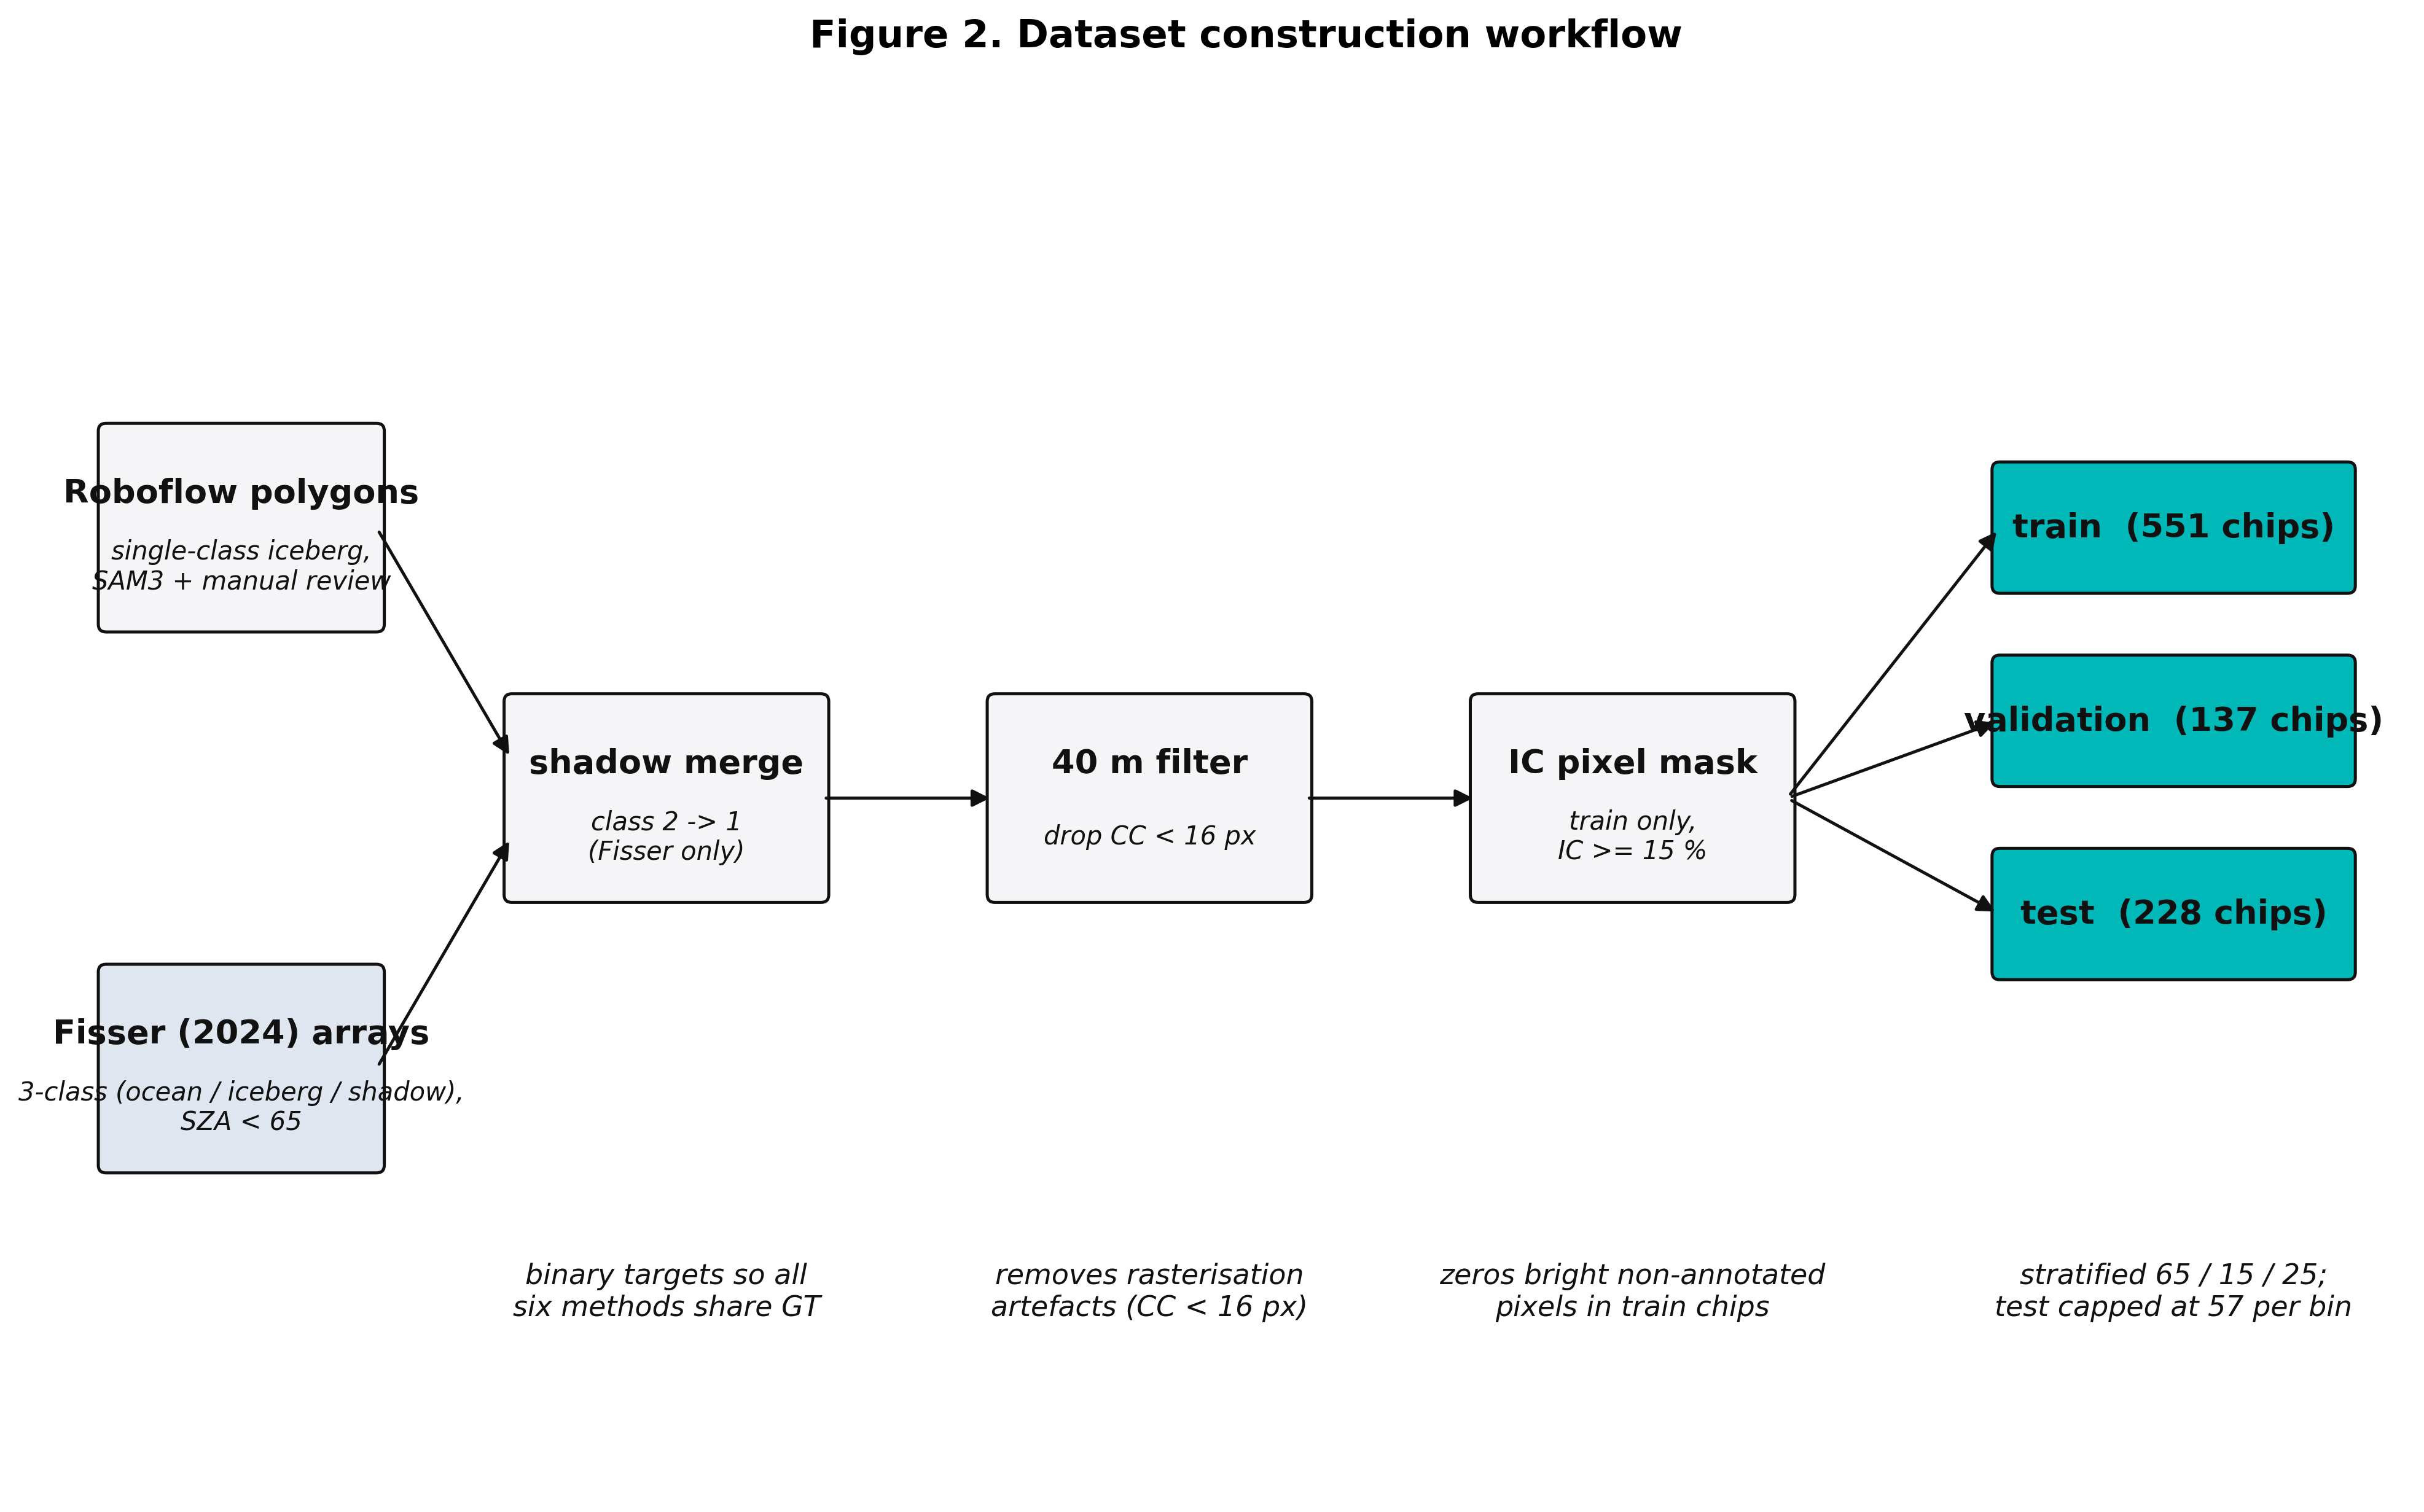
\includegraphics[width=\linewidth]{figures/fig-archive/20260505_150048__fig02_dataset_workflow.png}
\caption{\textbf{Fig. 2.} Dataset construction workflow. Two annotation sources are merged through three deterministic cleaning operations to produce the binary v4\_clean training, validation, and test splits. \textbf{Sources:} Roboflow polygons (single-class iceberg, SAM3 smart-select followed by manual review, SZA $\geq$ 65$^\circ$) and Fisser (2024) annotation arrays (3-class ocean / iceberg / shadow numpy arrays distributed as Python pickle files, SZA $<$ 65$^\circ$). \textbf{Cleaning operations, applied in order:} (1) \textit{shadow merge} - Fisser shadow pixels (class 2) are reclassified as iceberg (class 1) so every chip shares the same binary iceberg / non-iceberg target; (2) \textit{40 m component filter} - connected components below 16 pixels (40 m root length at the 10 m Sentinel-2 ground sample distance) are dropped from both sources to remove rasterisation artefacts and sub-resolution annotations; (3) \textit{annotation-aware ice-coverage (IC) pixel mask} - bright non-annotated pixels in training chips whose ice-coverage fraction is $\geq$ 15 \% are zeroed before training so the model does not learn that bright non-iceberg pixels (sea ice, melange) are negative examples. The IC mask applies only to training chips; validation and test chips are never masked. \textbf{Output:} a stratified 65 / 15 / 25 split yielding 551 train, 137 validation, and 228 test chips, with the test split capped at 57 chips per SZA bin.}
\label{fig:fig02_dataset_workflow}
\end{figure}

The working dataset is v4\_clean, materialised at \texttt{data/v4\_clean/manifest.json} and content-addressed by a single \texttt{chips\_sha} stamped into every downstream output. After the 40 m and IC filters, 916 chips survive: 330 from the \citet{Fisser2024} pickled set at SZA $<$ 65$^\circ$ (originally three-class: ocean, iceberg, shadow) and 586 chips annotated for this work at SZA $\geq$ 65$^\circ$ using a SAM3 smart-select tool followed by manual review. The Fisser shadow class is merged into iceberg before all analysis, producing the same binary label space as the Roboflow annotations: iceberg versus not-iceberg.

This binary convention is necessary for a fair combined-data experiment. It also reflects the area-retrieval task: shadowed faces attached to the iceberg are part of the above-water object even when their B08 reflectance is low. Merging the shadow class prevents the model from being asked to separate physical iceberg surface from adjacent iceberg shadow when the paper-level objective is iceberg segmentation.

The split target is 65 / 15 / 25 for training, validation, and testing. The materialised v4\_clean split is 551 training chips, 137 validation chips, and 228 test chips. The test set contains 57 chips per SZA bin, which keeps cross-bin comparisons from being dominated by the larger source bins. The 551 / 137 / 228 split is the one used for the canonical baseline\_v1 training and six-method reporting. The class distribution at the training-pixel level is binary: 94.4 \% ocean, 5.6 \% iceberg.

Two companion manifests support the controlled-variable design. v4\_raw is the same 984 source chips as v4\_clean materialised before the 40 m component filter and the annotation-aware IC pixel mask, with the same 65 / 15 / 25 split policy and seed (training count 592 vs. 551 in v4\_clean). v4\_raw\_lt65 is the lt65 subset of v4\_raw, restricted to the 398 \citet{Fisser2024} chips at SZA $<$ 65$^\circ$, and is the anchor manifest for Phase A's reference cell A0. The cleaned lt65 counterpart, v4\_clean\_lt65, contains the 330 lt65 chips that survive the 40 m and IC operations and is the anchor for Phase A's A2 cell. A null-injected variant (v4\_clean\_lt65\_plus\_nulls) adds GT0 chips at a 1:1 GT$+$ : GT0 ratio for the balancing experiments. The four lt65 manifests are derived from the same source chip pool and share split policy and seed, so the only variable that changes between Phase A cells is preprocessing or balancing rather than chip selection.


\section{Methods}

\begin{figure}[h]
\centering
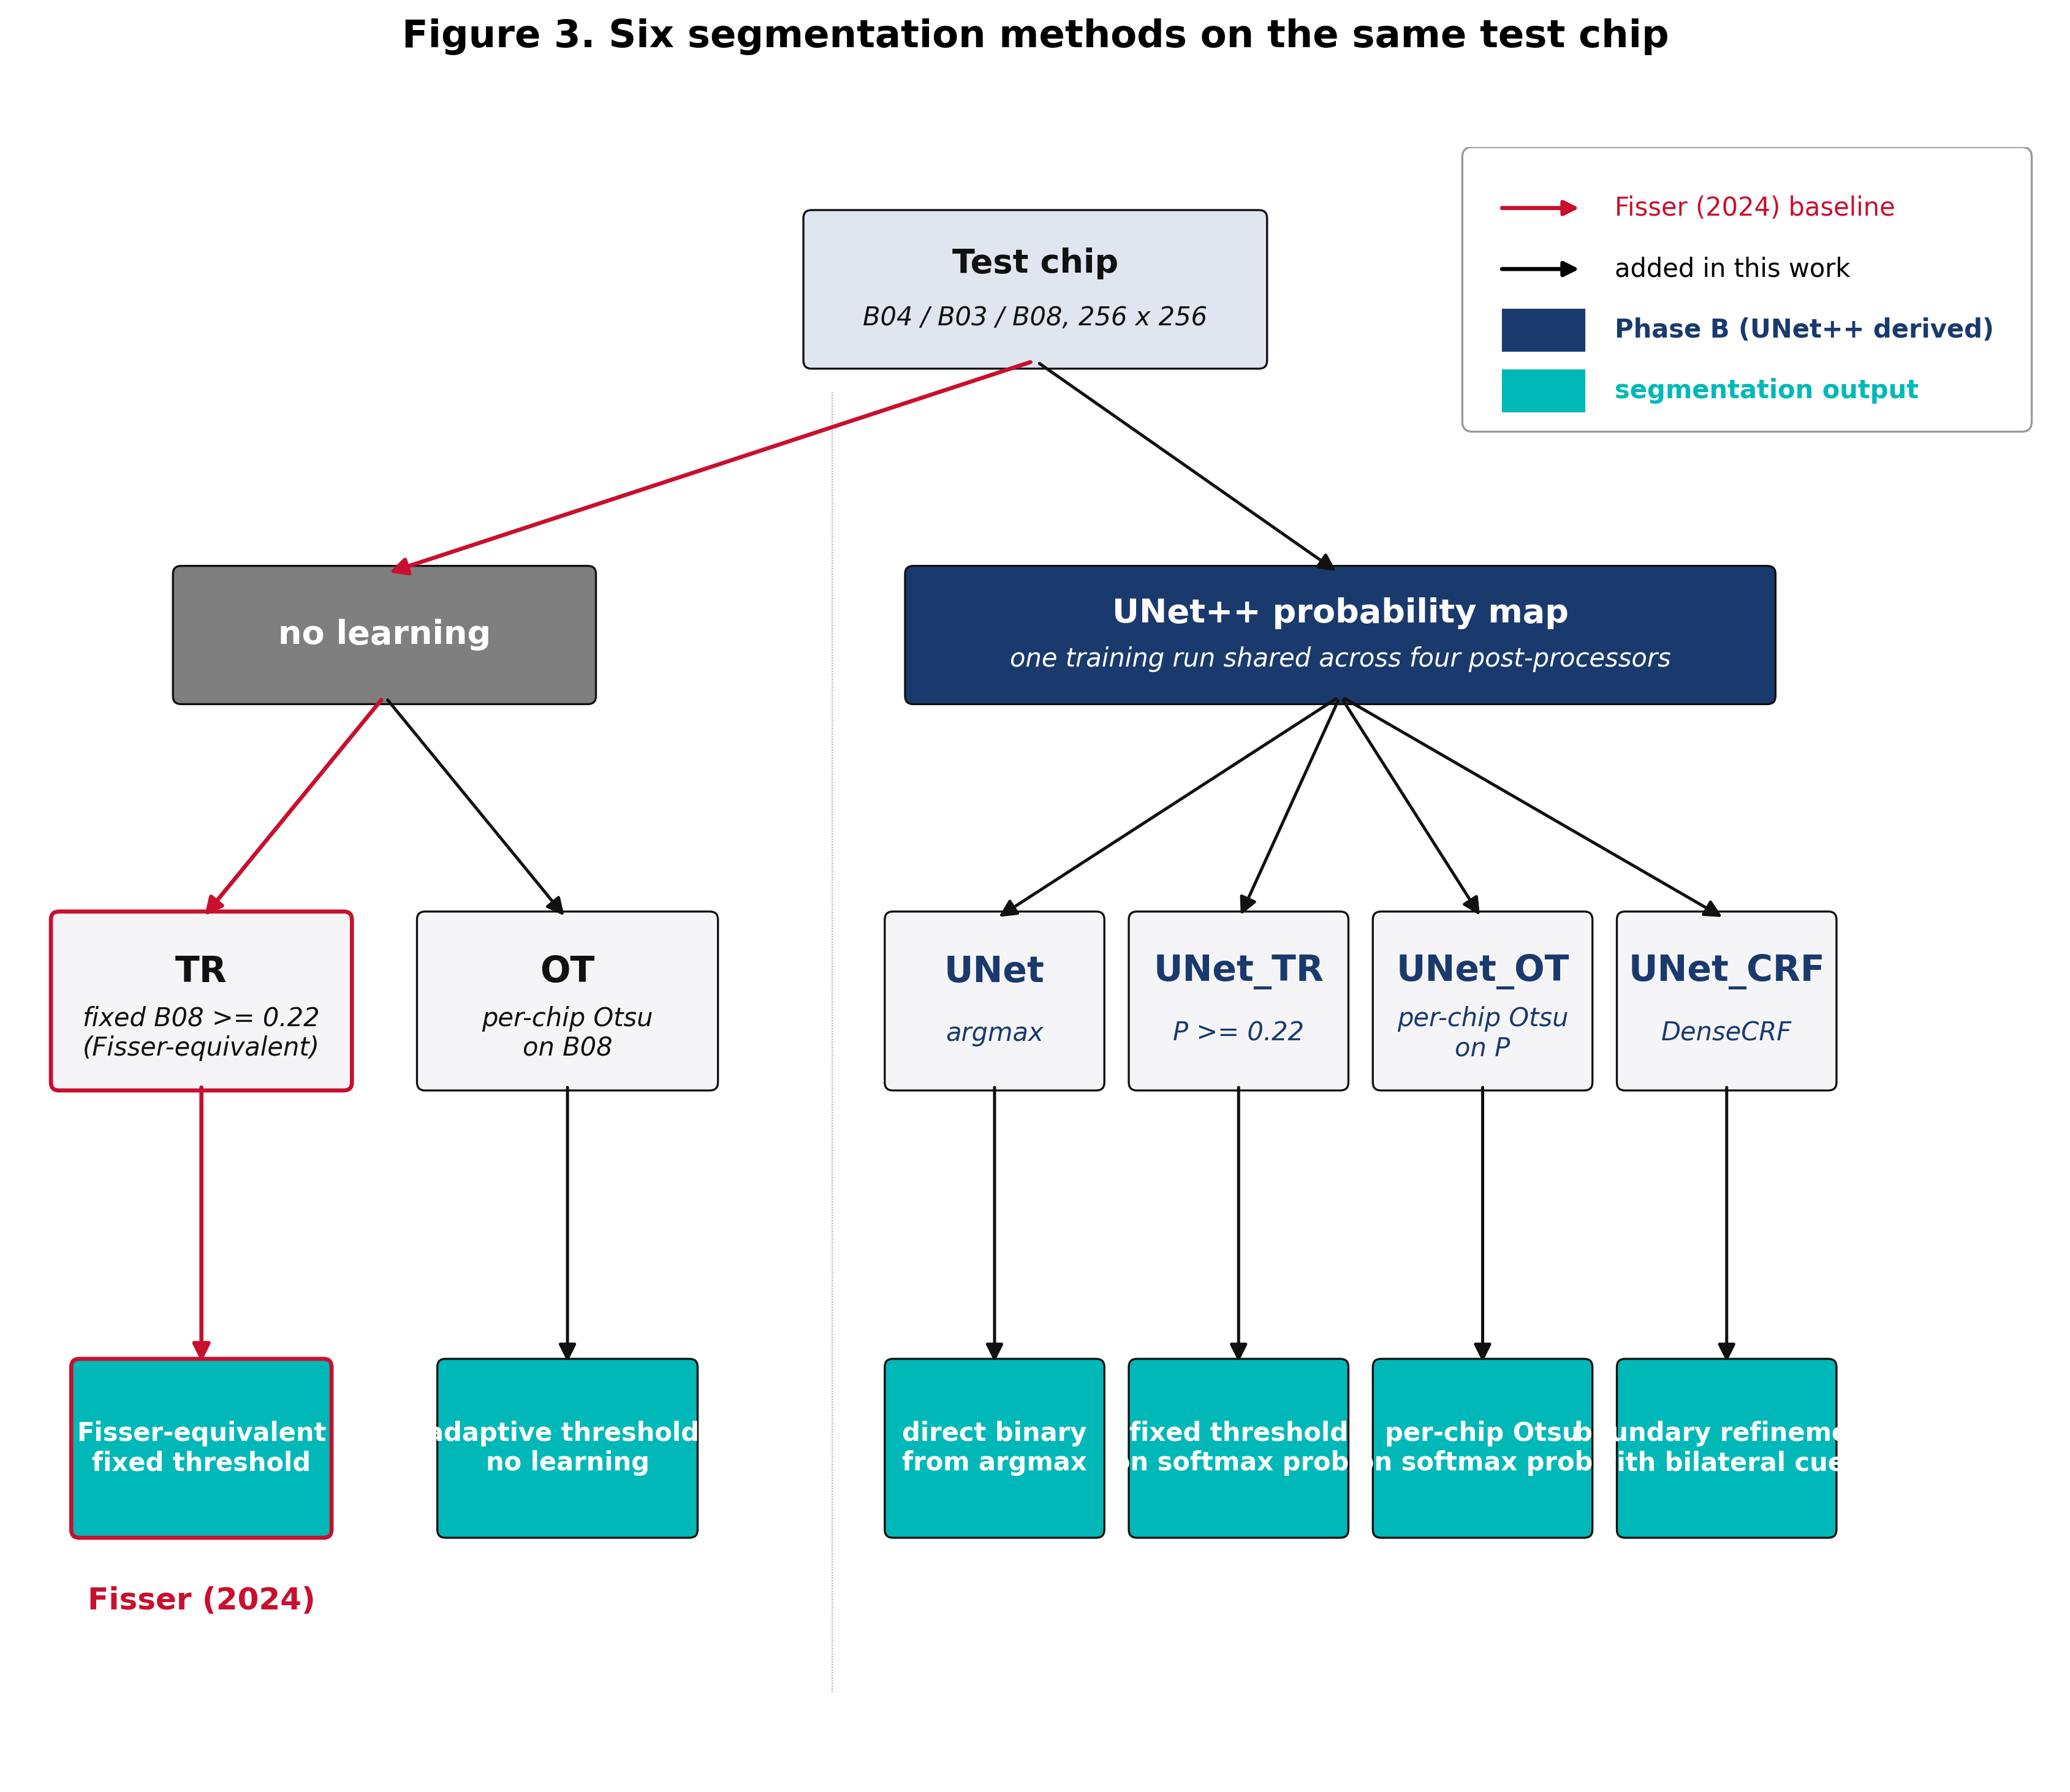
\includegraphics[width=\linewidth]{figures/fig-archive/20260505_151035__fig03_method_schematic.png}
\caption{\textbf{Fig. 3.} Six segmentation methods evaluated on the same test chip. Two methods operate directly on the input image (TR, OT). Four methods share the UNet++ probability map and differ only in post-processing (argmax, fixed threshold, per-chip Otsu, DenseCRF). One UNet++ training run produces all six method outputs. The TR path is drawn in red as the Fisser (2024) baseline; the OT branch and all four UNet++ post-processors are added in this work.}
\label{fig:fig03_method_schematic}
\end{figure}

\subsection{Six base segmentation pipelines}

The methods comparison begins with six base pipelines. The first two operate directly on the image. The third uses the learned segmentation map. The final three apply post-processing to the UNet++ probability surface. All six methods are evaluated on the same v4\_clean test chips.

\textbf{Fixed B08 threshold (TR).} A scene-wide B08 $\geq$ 0.22 cutoff applied per chip without spatial context. The 0.22 cutoff is the operational equivalent of the corrected-reflectance B08 $\geq$ 0.12 threshold reported by \citet{Fisser2024}, after the $+0.10$ uniform offset documented in Section 2.2 is preserved through the chip pipeline. Polygons below the 100 m$^2$ minimum area are discarded after polygonisation. TR also inherits an inference-time ice-coverage chip-skip filter: a chip is dropped from the prediction set if more than 15 \% of its pixels exceed B08 $\geq$ 0.22, on the assumption that pervasive bright pixels indicate sea-ice contamination rather than isolated icebergs. Skipped chips are recorded in the per-method audit log; their reference icebergs are counted as false negatives at evaluation rather than silently removed from the comparison. The chip-skip filter shares its 15 \% threshold with the training-time annotation-aware IC pixel mask (Section 2.3) but is operationally distinct: the pixel mask edits training chips, and the chip-skip filter rejects whole inference chips.

\textbf{Per-chip Otsu (OT).} A chip-adaptive threshold computed from the B08 histogram \citep{Otsu1979}, with guards on radiometrically flat or ice-contaminated chips (Otsu floor 0.10, ceiling 0.50). OT inherits the same inference-time chip-skip filter as TR. Provides an image-only adaptive baseline against which to measure the value of the fixed Fisser threshold under SZA shifts.

\textbf{UNet++ argmax (UNet).} The learned binary segmentation baseline. The model decision $P(\mathrm{iceberg}) > 0.5$ is applied to each pixel; the same model also saves the two-band probability raster used by the three downstream methods.

\textbf{UNet++ + threshold (UNet\_TR).} A fixed probability cutoff at $P(\mathrm{iceberg}) \geq 0.22$ on the saved UNet++ probability band. The 0.22 value matches the operational baseline\_v1 configuration; the same NIR-domain convention is applied to the softmax output to keep the threshold-based comparison anchored at one number.

\textbf{UNet++ + Otsu (UNet\_OT).} Per-chip Otsu computed on the UNet++ iceberg probability band rather than on raw B08 reflectance. Tests whether chip-adaptive thresholding gains accuracy when applied to a learned discriminant.

\textbf{UNet++ + DenseCRF (UNet\_CRF).} Dense conditional random field post-processing \citep{Krahenbuhl2011} on the UNet++ probability map plus image bands, encouraging spatially coherent boundaries aligned with image evidence (Gaussian sxy 3, compat 3; bilateral sxy 40, srgb 3, compat 4; 5 mean-field iterations).

\subsection{UNet++ training setup}

The learned model is a UNet++ \citep{Zhou2018} with a ResNet34 \citep{He2016} encoder pretrained on ImageNet. Inputs are 256 $\times$ 256 $\times$ 3 chips in B04 / B03 / B08 order; outputs are a single iceberg probability channel (binary segmentation). The canonical baseline\_v1 checkpoint was trained with seed 42 for 100 epochs on the 551 training chips of v4\_clean, with validation used only for checkpoint selection. A second checkpoint, A0, is trained under identical hyperparameters on v4\_raw\_lt65 (the 398 lt65 \citet{Fisser2024} chips with no 40 m filter and no IC pixel mask) and serves as the lt65 anchor for the Fisser-comparable subset of the method sweep. baseline\_v1 carries the headline four-bin tables; A0 carries the lt65 direct-comparison cell.

The optimisation objective is Dice plus binary cross-entropy. AdamW \citep{Loshchilov2019} drives optimisation with learning rate $1 \times 10^{-4}$, weight decay $1 \times 10^{-4}$, batch size 16, and cosine learning-rate scheduling. Random horizontal flips, vertical flips, and 90$^\circ$ rotations are enabled. The training script requires an explicit seed when an experiment-mode environment variable is set, and output artefacts are stamped with manifest and configuration identifiers to prevent cross-run drift.

\subsection{White top-hat small-iceberg recovery}

White top-hat morphological filtering is the recovery extension applied uniformly to all six base methods, producing six $+$TH variants. For each chip the top-hat response is computed on the B08 band with a disk structuring element of radius 10 pixels (100 m), thresholded at 0.05 reflectance units, filtered to connected components $\geq$ 16 pixels, and unioned with the base method's polygons. Pixels already covered by the base prediction are excluded from the recovery candidate set, so the top-hat output adds missed candidates rather than redrawing detections the base method already found. Top-hat is post-inference only and does not retrain or modify the UNet++ checkpoint.

\subsection{Evaluation}

\begin{figure}[h]
\centering
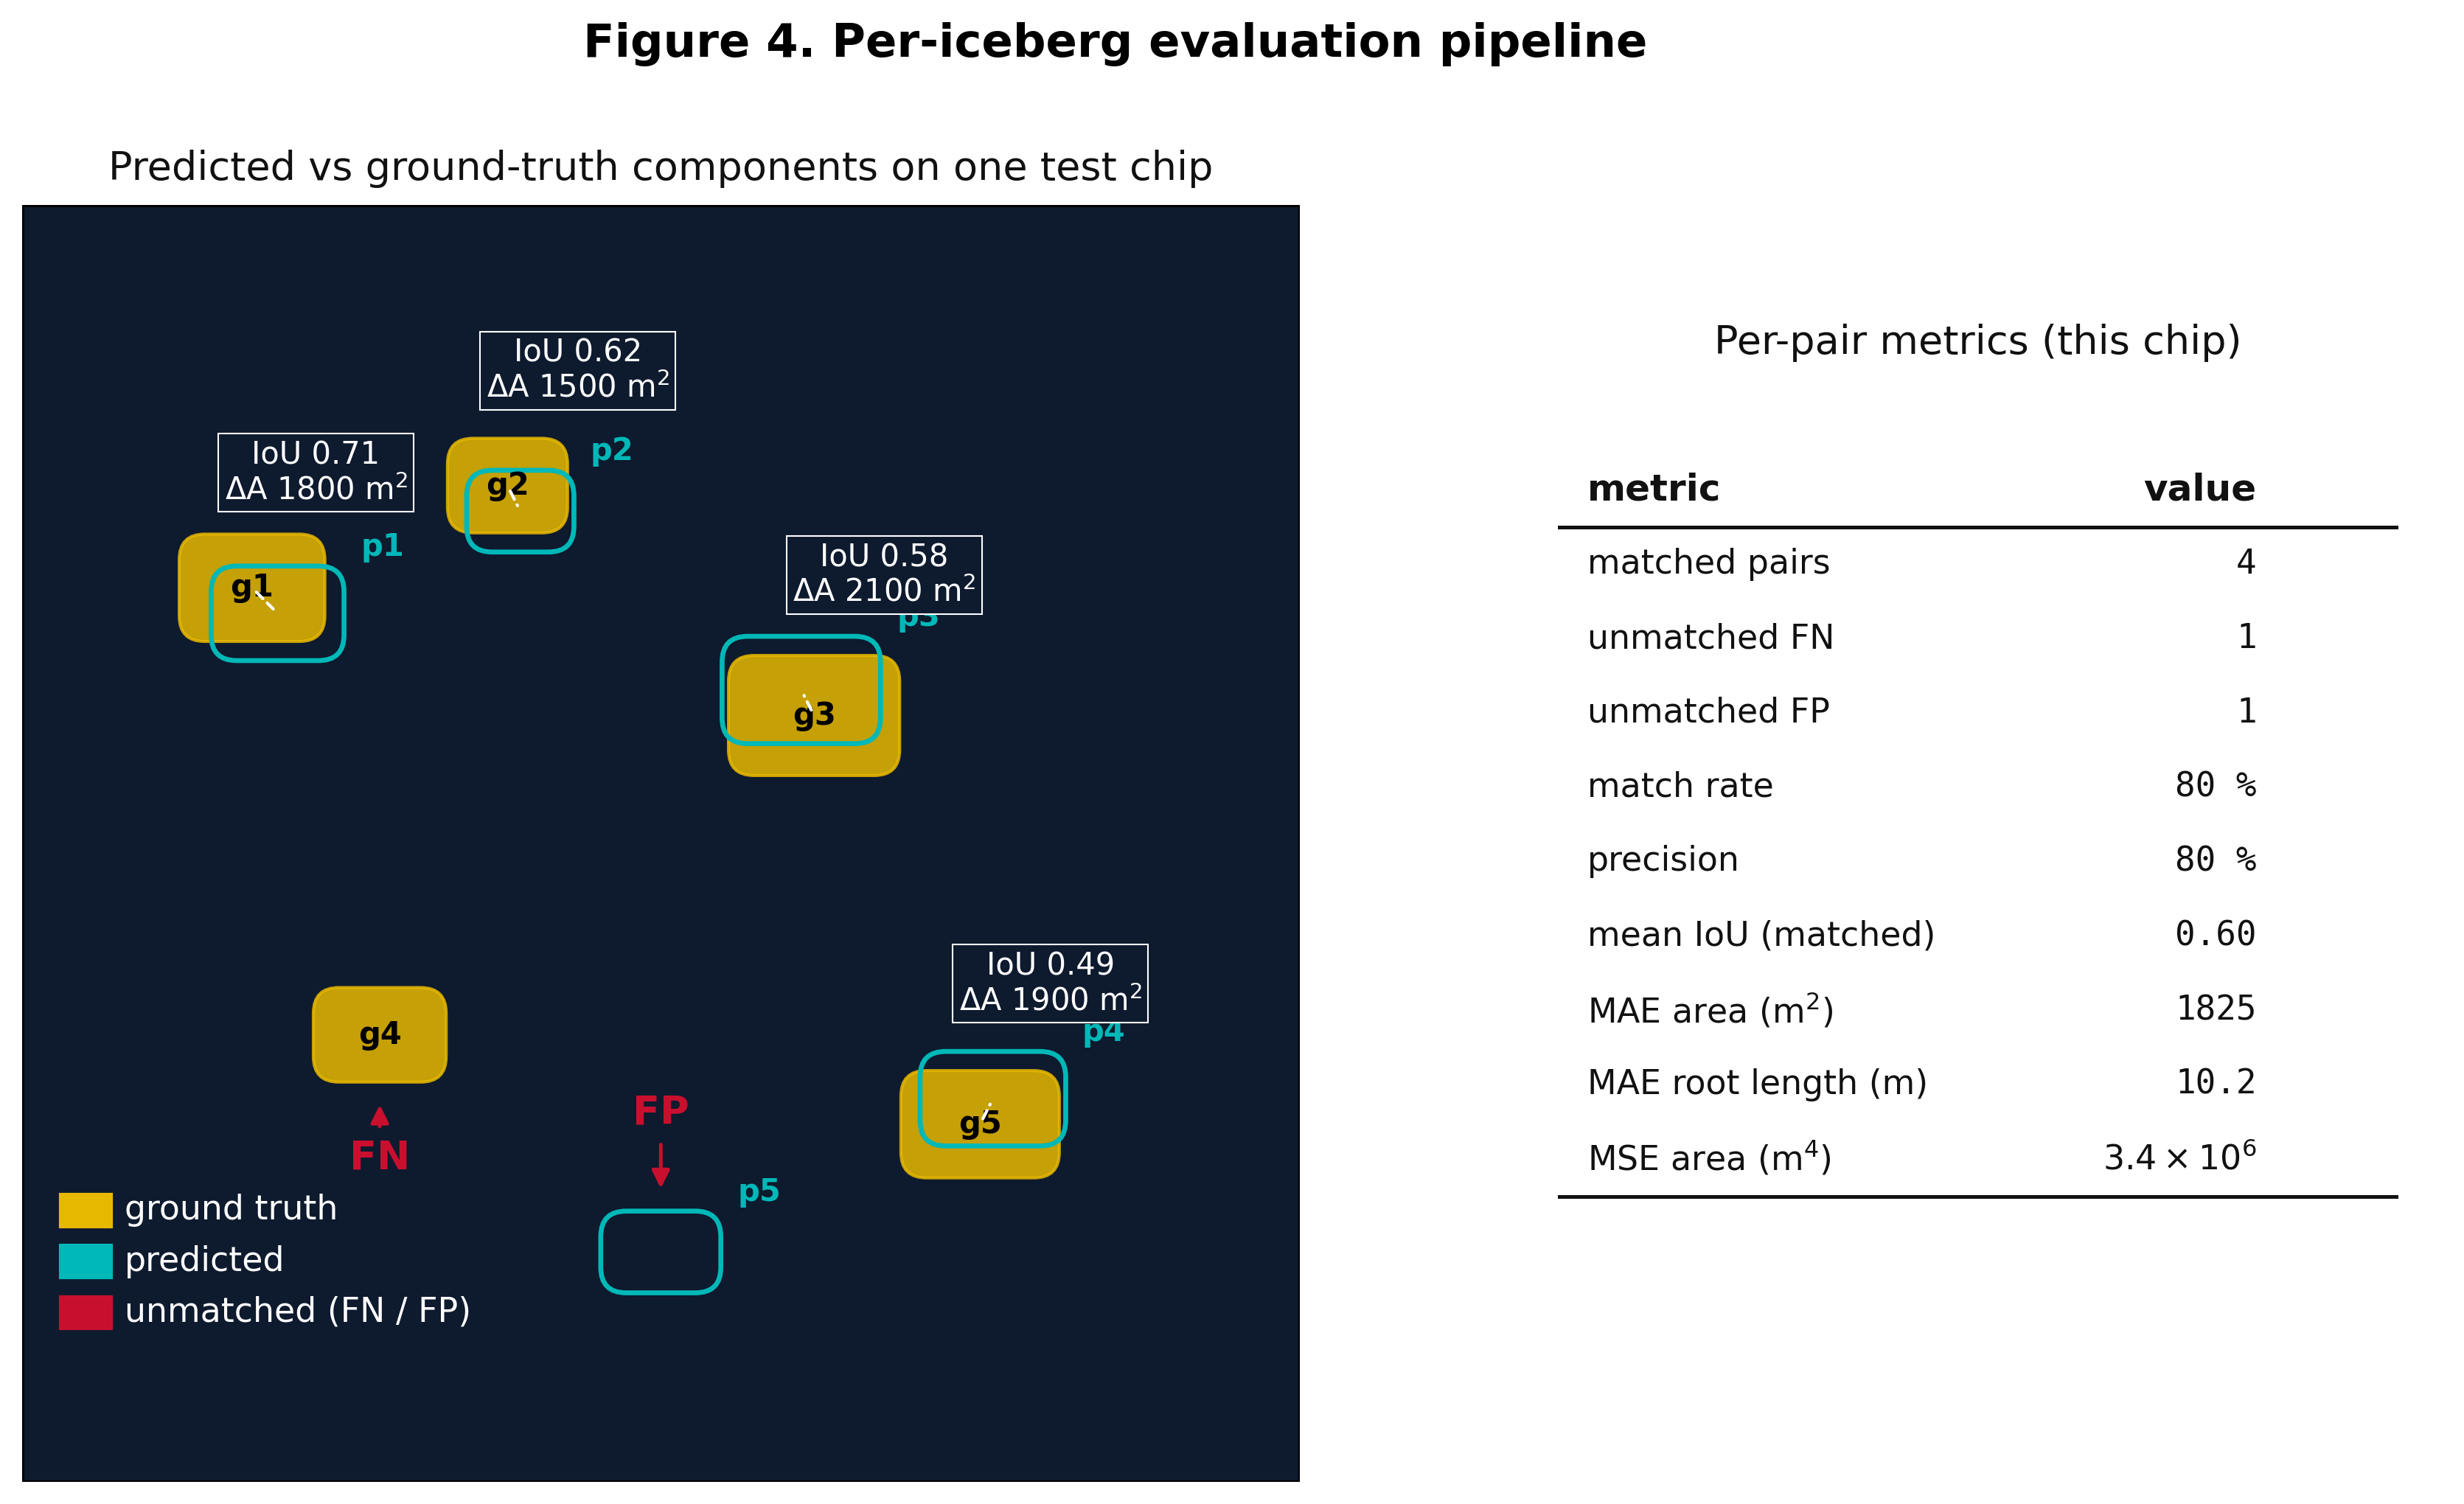
\includegraphics[width=\linewidth]{figures/fig-archive/20260505_145113__fig04_evaluation_schematic.png}
\caption{\textbf{Fig. 4.} Per-iceberg evaluation pipeline. Ground-truth components and predicted components are matched by Hungarian assignment on $(1 - \mathrm{IoU})$, keeping pairs with $\mathrm{IoU} \geq 0.30$. Unmatched components count as false negatives or false positives in the detection table; matched pairs feed mean absolute error on area, mean absolute error on root length, mean IoU, and the area MSE reported per (method, SZA bin) cell.}
\label{fig:fig04_evaluation_schematic}
\end{figure}

Evaluation is organised around area retrieval because that is the scientific quantity shared with the threshold literature. Predictions are polygonised into one feature per detected iceberg and rasterised back to the chip grid for comparison with the binary ground-truth mask. Two evaluation views are produced: chip-level segmentation metrics and per-iceberg matched-pair metrics.

The headline metric is mean absolute error (MAE) on matched iceberg area and on square-root area, used as a root-length proxy. MAE is primary because it is interpretable in physical units and is the closest bridge to Fisser-style area-error reporting. Intersection over union (IoU) is reported second on matched pairs for segmentation-community comparison. Mean squared error (MSE) is supplementary because it heavily weights large outliers but remains useful for diagnosing area-error variance. For predicted mask $P$ and reference mask $R$,
\begin{equation}
\mathrm{IoU} = \frac{|P \cap R|}{|P \cup R|} = \frac{\mathrm{TP}}{\mathrm{TP} + \mathrm{FP} + \mathrm{FN}}.
\label{eq:iou}
\end{equation}

Predicted and reference iceberg areas are computed from polygonised or rasterised masks; for chip $i$,
\begin{equation}
A_{\mathrm{pred}, i} = n_{\mathrm{pred}, i} \cdot r^2, \qquad A_{\mathrm{ref}, i} = n_{\mathrm{ref}, i} \cdot r^2,
\label{eq:chip_area}
\end{equation}
where $r = 10$ m is the Sentinel-2 pixel size. The signed per-chip area error $e_i = A_{\mathrm{pred}, i} - A_{\mathrm{ref}, i}$ feeds the chip-level error statistics across $N$ evaluated chips:
\begin{equation}
\mathrm{MAE}_{\mathrm{area}} = \frac{1}{N} \sum_i |e_i|, \qquad \mathrm{MSE}_{\mathrm{area}} = \frac{1}{N} \sum_i e_i^2.
\label{eq:chip_mae_mse}
\end{equation}

For the per-iceberg matched-pair tables, ground-truth and predicted connected components are paired by Hungarian assignment on $1 - \mathrm{IoU}$, keeping only pairs whose IoU exceeds the threshold $\tau = 0.30$. For $M$ matched pairs $(j)$,
\begin{equation}
\mathrm{MAE}_{\mathrm{root}} = \frac{1}{M} \sum_j \left| \sqrt{A_{\mathrm{pred}, j}} - \sqrt{A_{\mathrm{ref}, j}} \right|,
\label{eq:pair_mae_root}
\end{equation}
with the analogous per-pair MAE on area and per-pair IoU on the matched subset. Unmatched components count as false negatives or false positives in the detection table. Each method therefore reports not only MAE and IoU but also detection counts, match rate, and precision so that low-error results on a small matched subset are not over-interpreted.

\subsection{Experiment progression and reproducibility}

The paper is structured as a controlled progression rather than a flat method leaderboard. Phase A walks the dataset axis using lt65-scoped experiments. The reference cell A0 anchors on v4\_raw\_lt65 (398 lt65 chips, no 40 m filter, no IC mask, faithful to Fisser's published preprocessing). A2 anchors on v4\_clean\_lt65 (330 chips, our 40 m and IC pipeline applied), and A1, A3 through A9 walk null-chip injection, augmentation, and class plus size balancing schemes from these two anchors. Each step changes one controlled variable, declared by a \texttt{controlled\_variable} field in the experiment YAML so the comparison cannot drift. Phase B walks the method axis on a frozen training checkpoint, producing all six base method outputs from a single training run. The headline four-bin tables run on baseline\_v1 (v4\_clean, all SZA bins); the lt65 Fisser-comparable cell is run a second time on the A0 checkpoint and the v4\_raw\_lt65 test split, to keep the SZA $<$ 65$^\circ$ comparison free of the 40 m and IC interventions. Top-hat recovery is evaluated as a uniform post-inference extension to those base outputs.

Every experiment is driven through the same five named stages (manifest, train, infer, evaluate, figures). The manifest carries a \texttt{chips\_sha} content hash, and downstream outputs stamp the experiment id, manifest hash, configuration hash, seed, and code commit. These stamps make cross-experiment comparisons grounded in byte-identical chip membership.

The current paper deliberately holds the model architecture and input channel set fixed. The contribution is a controlled evaluation of dataset cleaning, dataset extension into high-SZA scenes, six base segmentation pipelines, and white top-hat recovery under one reproducible pipeline. Architecture variants and covariate-informed classifiers (CatBoost, contrast-based modelling, dynamic thresholding) are scoped as future extensions and have no trained model, inference outputs, or evaluation tables in this paper.


\section{Results}

\begin{figure*}[h]
\centering
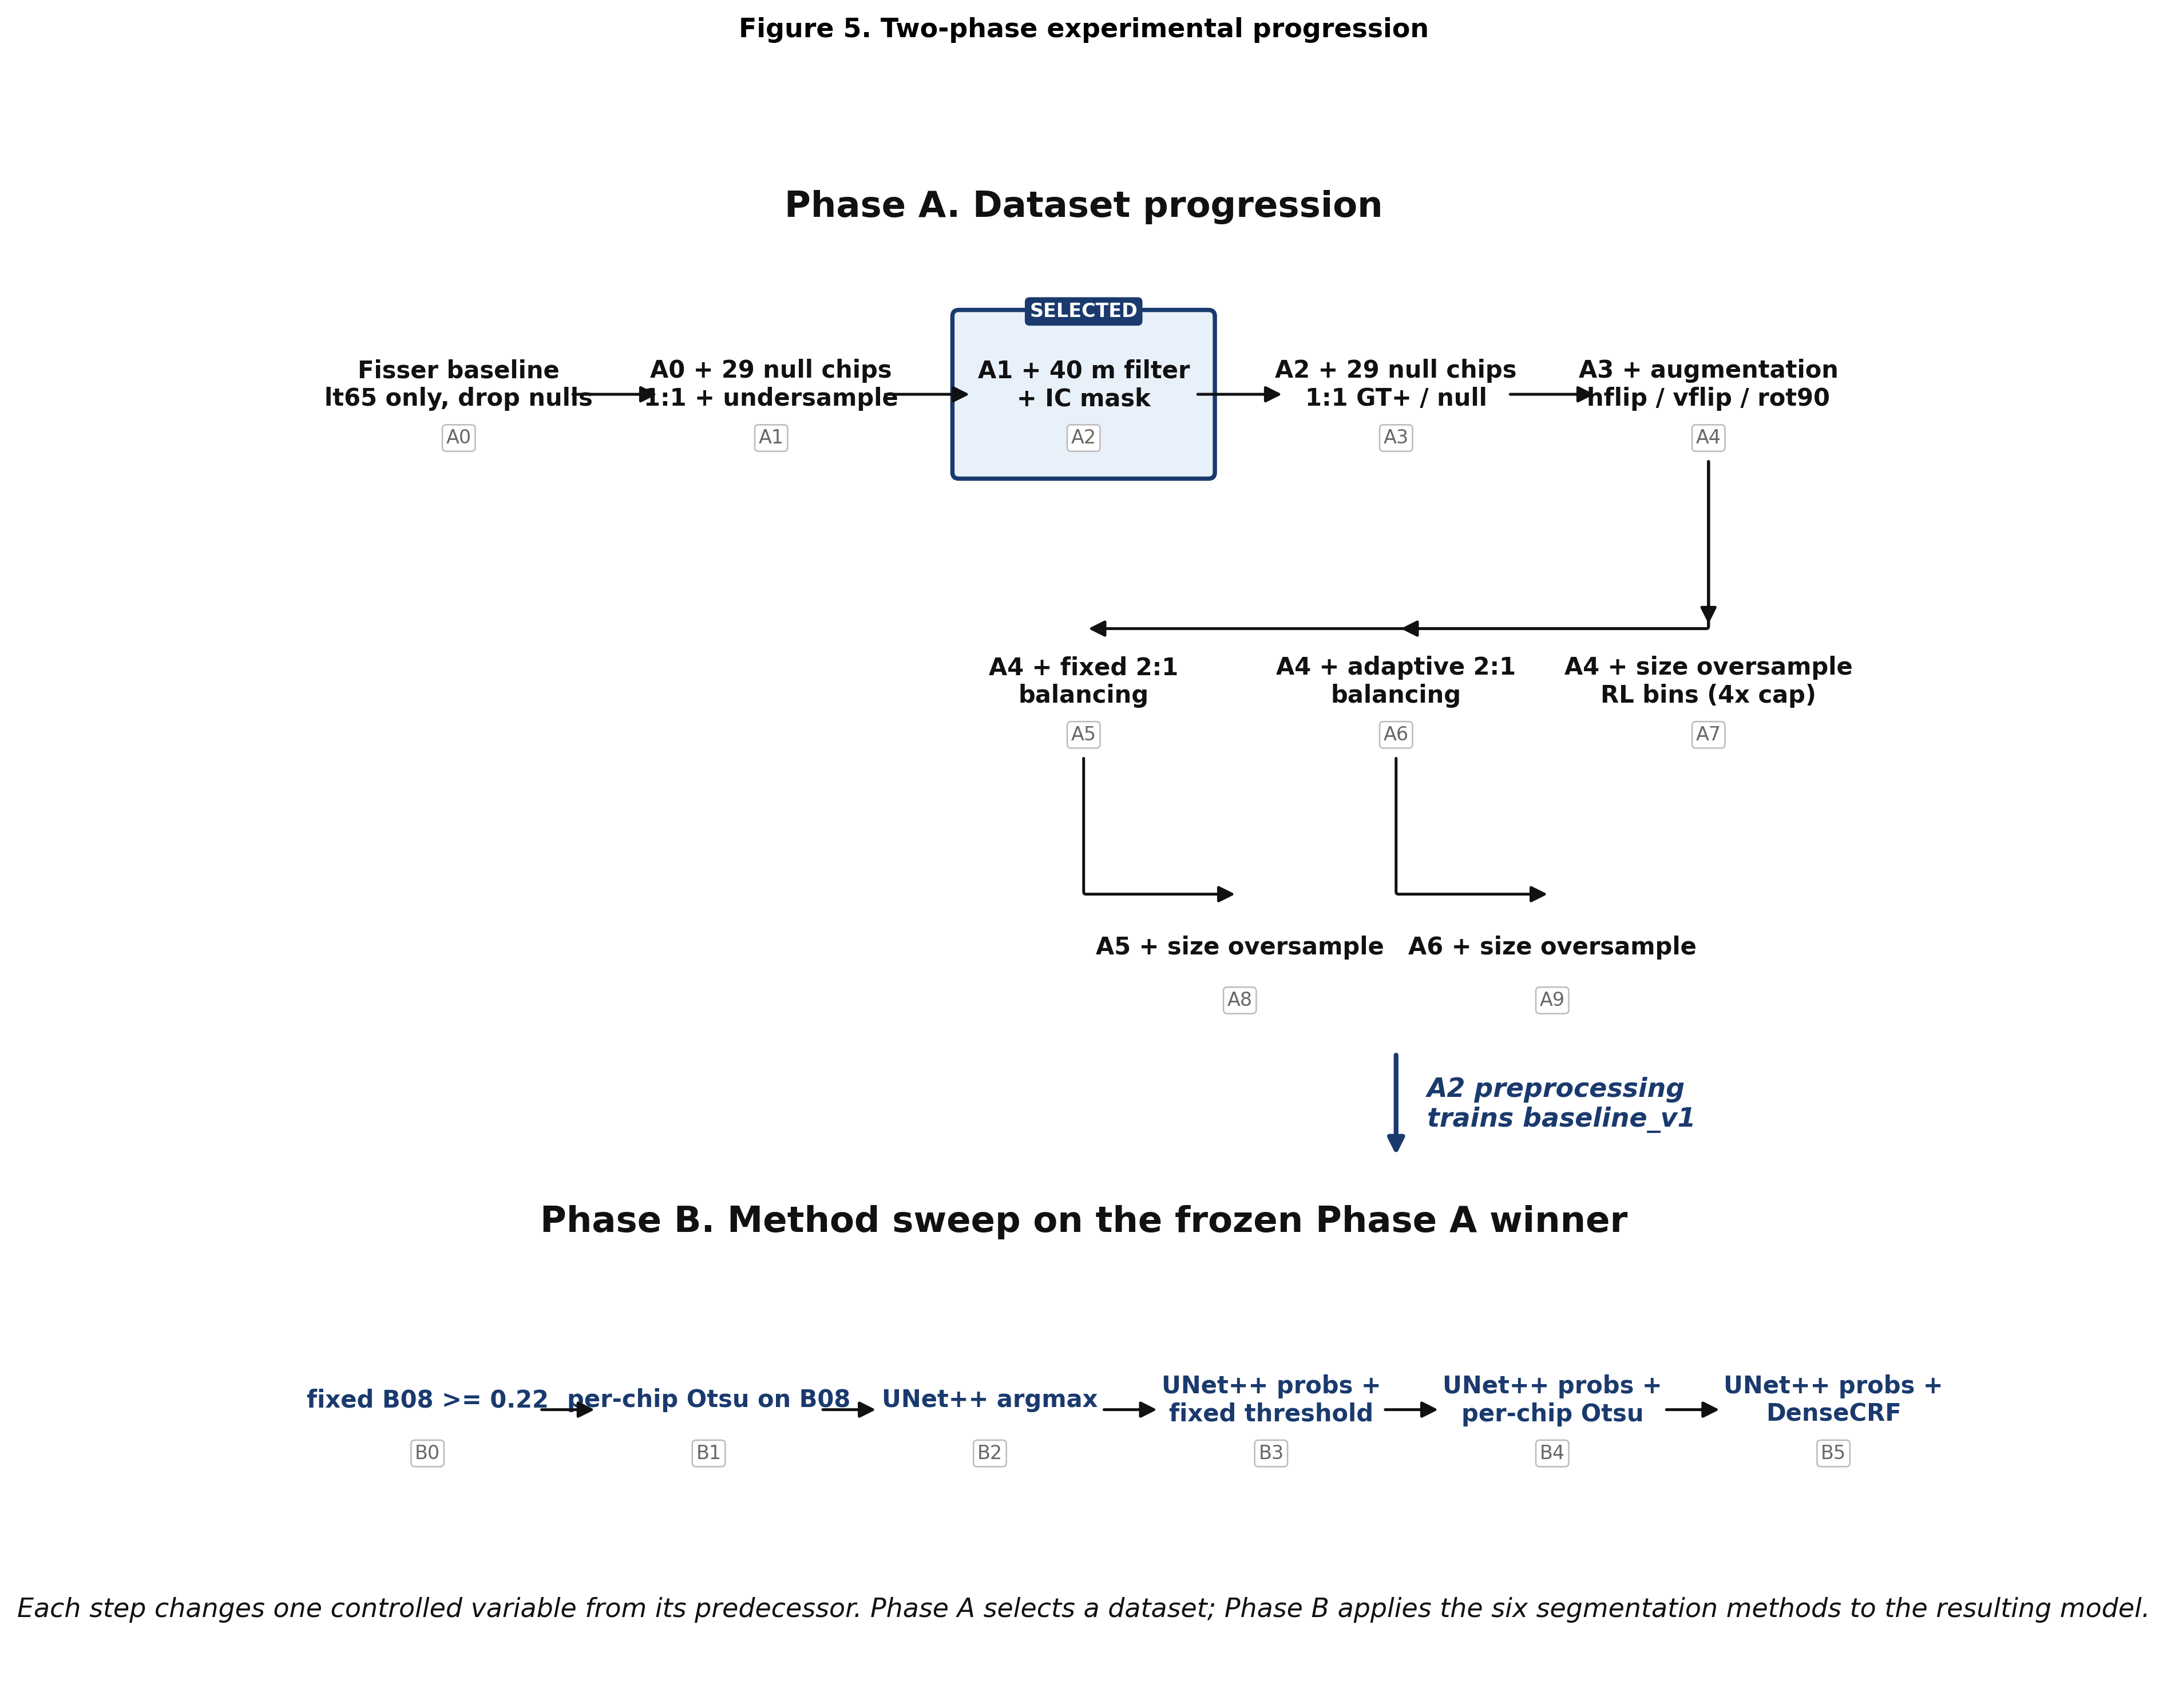
\includegraphics[width=\textwidth]{figures/fig-archive/20260505_151537__fig05_progression.png}
\caption{\textbf{Fig. 5.} Two-phase experimental progression. Phase A walks the dataset axis, isolating one cleaning or balancing variable per step. The selected dataset is frozen and passed to Phase B, which sweeps the six segmentation methods of Fig.~\ref{fig:fig03_method_schematic} in a single inference dispatch. Each step's motivation is reader-facing; implementation details (manifest identifiers, balancing-scheme labels, training hyperparameters) are deferred to the methods text.}
\label{fig:fig05_progression}
\end{figure*}

\subsection{Per-iceberg metrics on the canonical baseline}

Table 1 reports per-pair root-length mean absolute error, computed by Hungarian matching on $1 - \mathrm{IoU}$ with a post-filter $\mathrm{IoU} \geq 0.30$, on the v4\_clean test split (\textit{n} = 228 chips, 7,201 reference icebergs). The UNet++ + DenseCRF combination wins three of four SZA bins; UNet++ + Otsu wins the lt65 bin. Threshold-only methods (TR, OT) degrade as SZA rises, while the learned methods stay flat across bins. Fig.~\ref{fig:mae_rootlen_vs_sza} renders the same data as a column chart with per-bin pair counts annotated.

\begin{figure}[h]
\centering
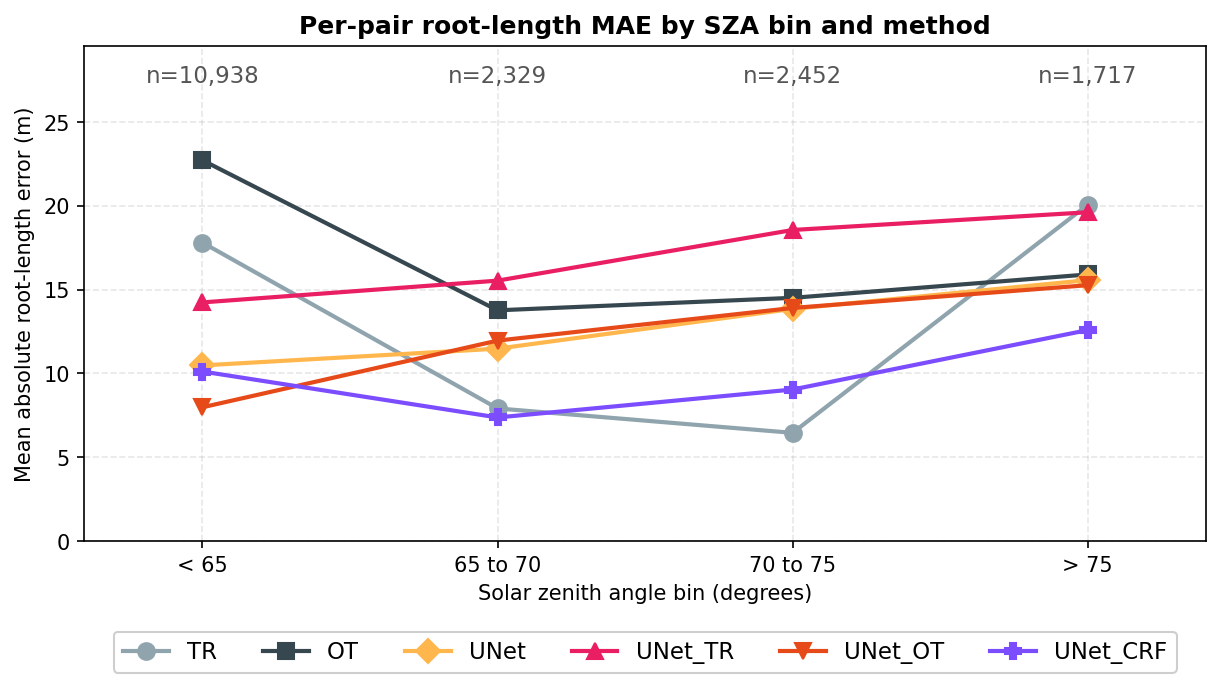
\includegraphics[width=0.95\linewidth]{figures/fig-archive/20260505_152446__mae_rootlen_vs_sza.png}
\caption{\textbf{Fig. 6.} Per-pair mean absolute root-length error by SZA bin and method, from Hungarian-matched reference vs predicted iceberg pairs in the v4\_clean test split. Per-bin n\textsubscript{pairs} annotated near the top of each column. Fisser (2024) Fig. 11 analog.}
\label{fig:mae_rootlen_vs_sza}
\end{figure}

\begin{table}[h]
\caption{\textbf{Table 1.} Per-pair mean absolute error of iceberg root length (m) on the v4\_clean test split. Lower is better. Bold marks the best method per SZA bin.}
\centering
\begin{tabular}{lrrrr}
\toprule
Method & $<$ 65$^\circ$ & 65--70$^\circ$ & 70--75$^\circ$ & $>$ 75$^\circ$ \\
\midrule
TR\textsuperscript{a} & 17.8           & 7.9            & 6.5            & 20.1 \\
OT        & 22.7           & 13.8           & 14.5           & 15.9 \\
UNet      & 10.5           & 11.5           & 13.9           & 15.6 \\
UNet\_TR  & 14.2           & 15.5           & 18.6           & 19.6 \\
UNet\_OT  & \textbf{8.0}   & 12.0           & 13.9           & 15.3 \\
UNet\_CRF & 10.1           & \textbf{7.4}   & \textbf{9.0}   & \textbf{12.6} \\
\bottomrule
\end{tabular}\\
\smallskip
\footnotesize\textsuperscript{a}TR threshold = 0.22 in our radiometric units, which equals the Fisser (2024) published value of 0.12 after correcting for the +0.10 DN offset our pipeline preserves (Section 2.7). The TR row is the explicit Fisser-threshold reproduction.
\end{table}

Table 2 reports per-pair mean Intersection over Union on matched pairs. UNet++ + Otsu leads in lt65; UNet++ + DenseCRF leads in 65--70$^\circ$; UNet++ alone leads in higher SZA bins. Fig.~\ref{fig:area_scatter} renders predicted vs reference iceberg area as a per-SZA-bin scatter with all six methods overlaid: cool blue-grey tones mark non-learning methods (TR, OT) and learning methods are differentiated by both color and marker shape (UNet light orange, UNet\_TR pink, UNet\_OT red, UNet\_CRF bright purple). The 1:1 line is solid black; a shaded $\pm$25\% band marks the over- and under-estimation regions. Each panel insets a per-method match rate (matched pairs over total reference icebergs in the panel) and MAE on iceberg root length, so the inset values cross-reference Table 1 and Table 3 directly.

\begin{figure}[h]
\centering
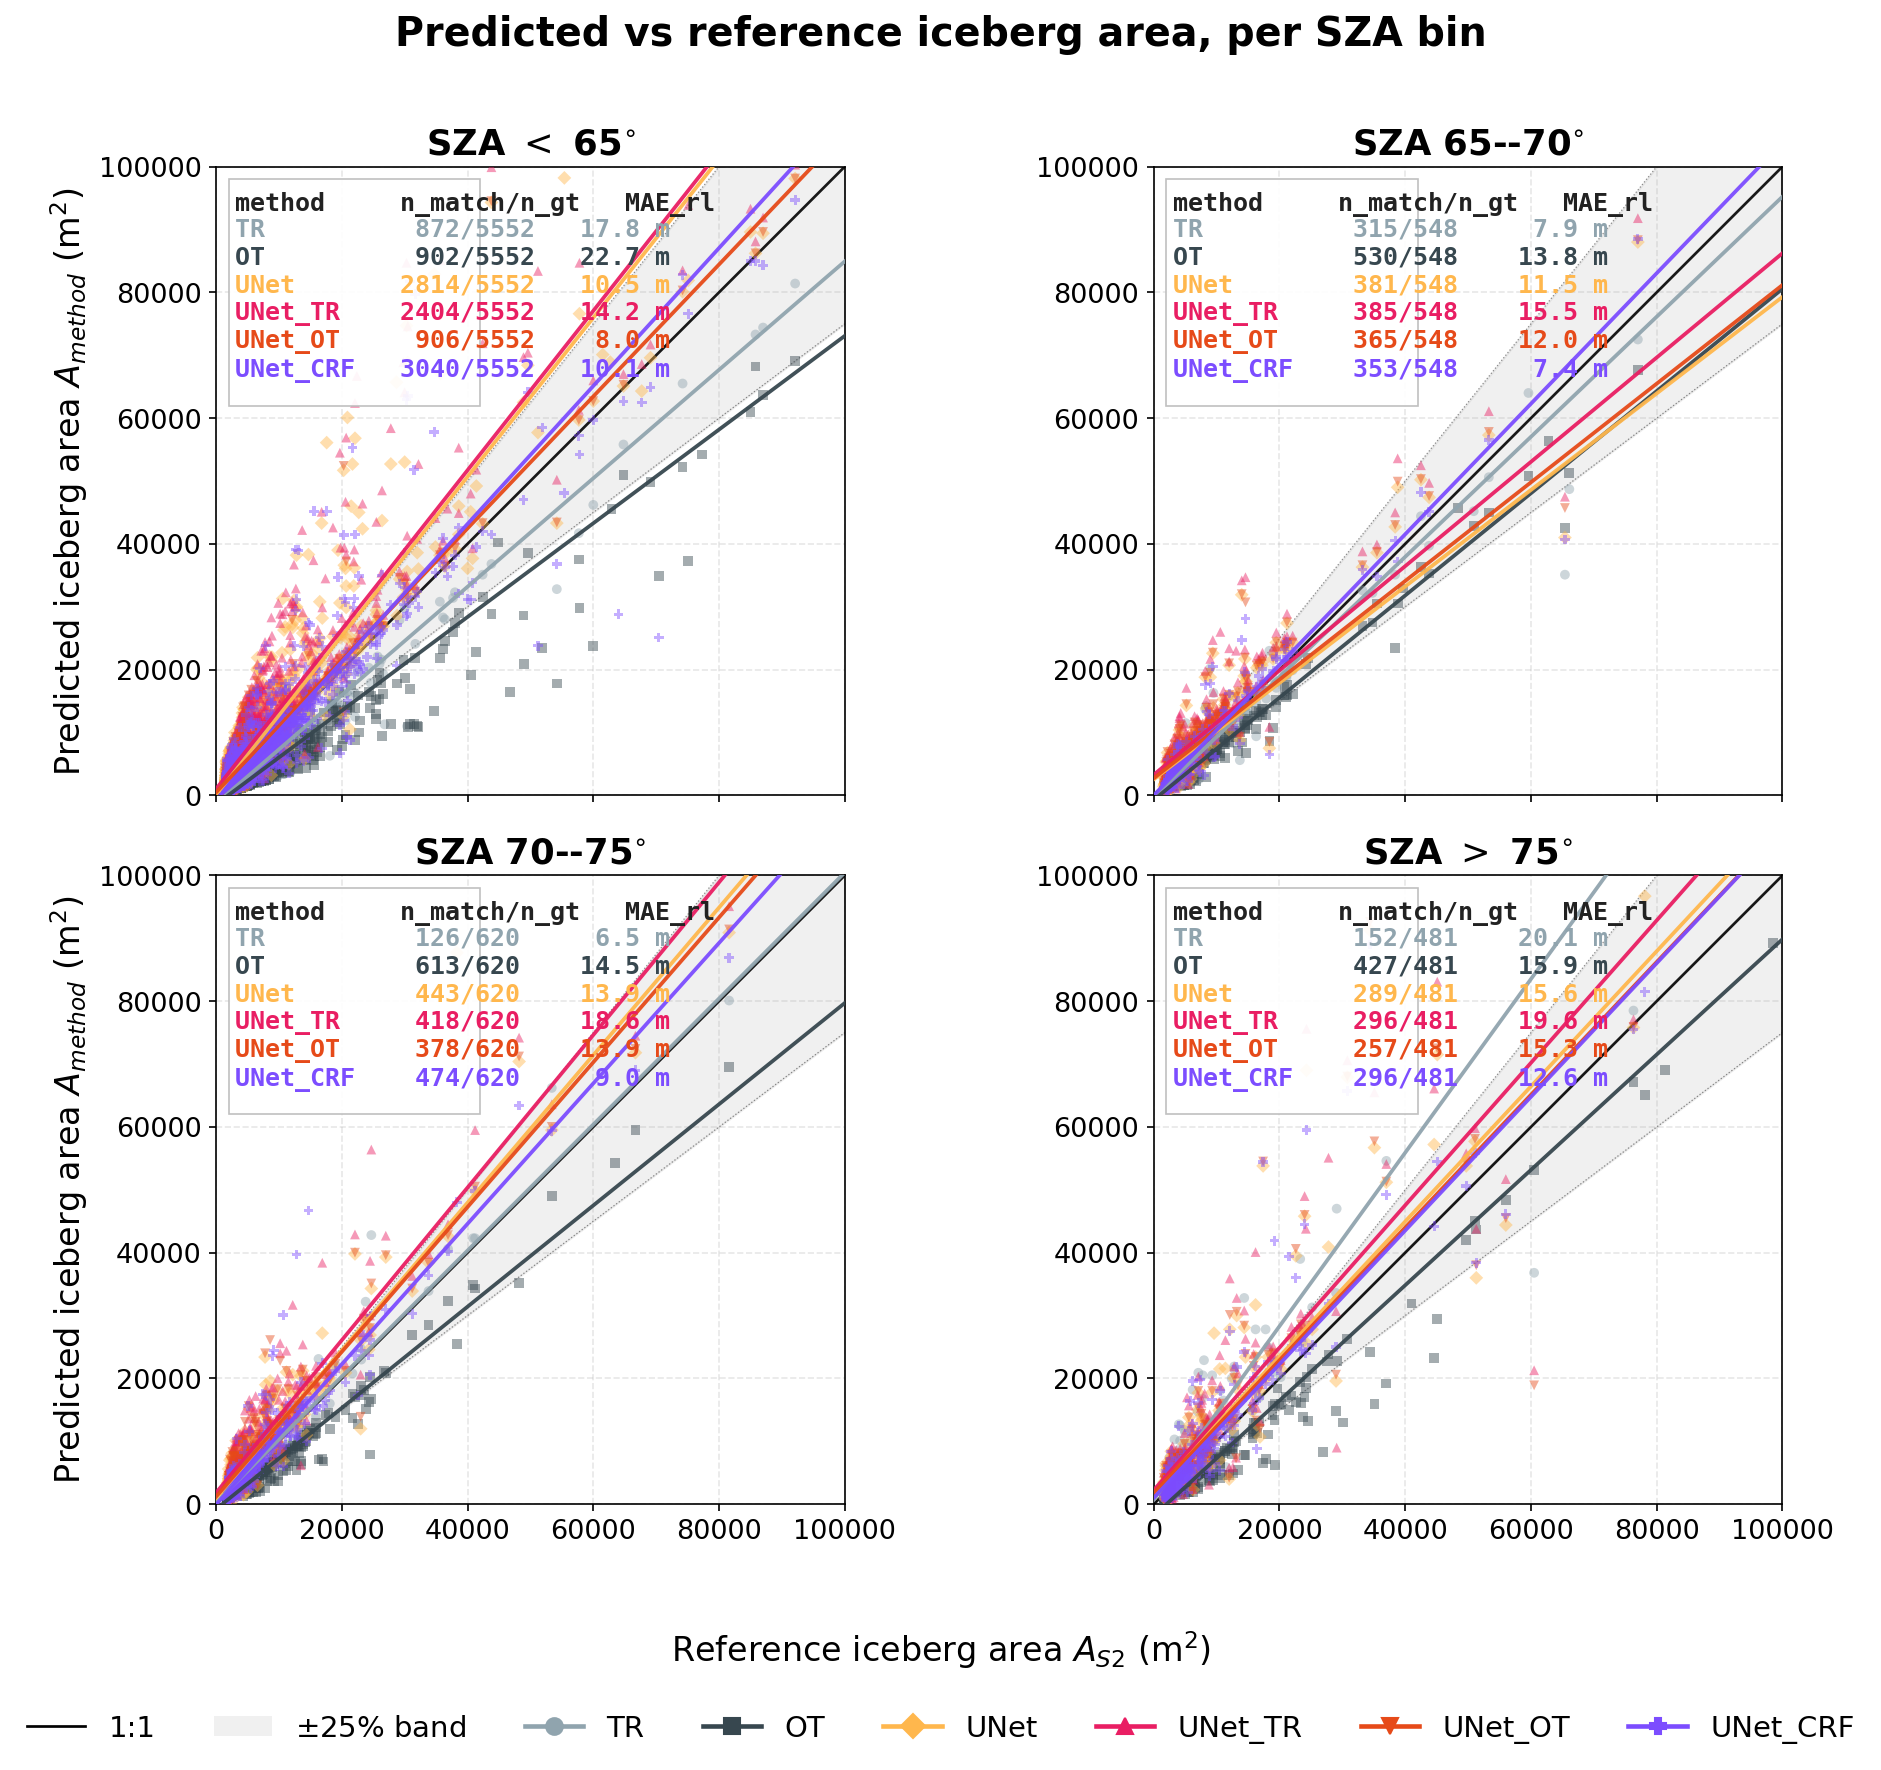
\includegraphics[width=0.95\linewidth]{figures/fig-archive/20260505_153322__area_scatter_by_method.png}
\caption{\textbf{Fig. 7.} Per-pair predicted vs reference iceberg area, one panel per SZA bin, with the 1:1 line solid black and a shaded $\pm$25\% band marking over- and under-estimation regions. Each method overlays a colored point cloud and matching-color OLS fit line; method shapes additionally differ (TR circle, OT square, UNet diamond, UNet\_TR up-triangle, UNet\_OT down-triangle, UNet\_CRF plus) so the same method is identifiable across Fig.~\ref{fig:bias_delta_by_area} and Fig.~\ref{fig:re_by_area_bin}. Cool blue-grey tones mark non-learning methods (TR, OT); learning methods are UNet light orange, UNet\_TR pink, UNet\_OT red, UNet\_CRF bright purple. Inset table reports per-method n\_matched / n\_gt (matched pairs over total reference icebergs in the panel; the ratio equals the match rate / recall in Table 3) and MAE on iceberg root length (m), matching Fig.~\ref{fig:mae_rootlen_vs_sza} and Table 1 entries for the same SZA bin. Fisser (2024) Fig. 6 / Fisser (2025) Fig. 10 analog.}
\label{fig:area_scatter}
\end{figure}

\begin{table}[h]
\caption{\textbf{Table 2.} Per-pair mean IoU on matched iceberg pairs, v4\_clean test split. Higher is better. Bold marks the best method per SZA bin.}
\centering
\begin{tabular}{lrrrr}
\toprule
Method & $<$ 65$^\circ$ & 65--70$^\circ$ & 70--75$^\circ$ & $>$ 75$^\circ$ \\
\midrule
TR        & 0.48           & 0.67           & 0.69           & 0.59 \\
OT        & 0.47           & 0.62           & 0.62           & 0.62 \\
UNet      & 0.70           & 0.67           & 0.64           & 0.65 \\
UNet\_TR  & 0.66           & 0.64           & 0.60           & 0.61 \\
UNet\_OT  & \textbf{0.73}  & 0.67           & 0.64           & 0.64 \\
UNet\_CRF & 0.65           & \textbf{0.69}  & \textbf{0.67}  & \textbf{0.66} \\
\bottomrule
\end{tabular}
\end{table}

Table 3 reports detection statistics (the selection-bias disclosure required for cross-method MAE comparison). UNet++ + DenseCRF achieves the highest match rate (57.8\%); threshold-only methods match fewer than 35\% of reference icebergs, so their lower MAE in some bins reflects easier-to-match icebergs rather than across-the-board accuracy. Fig.~\ref{fig:bias_delta_by_area} decomposes per-pair bias by reference iceberg area, and Fig.~\ref{fig:re_by_area_bin} reports the per-pair relative error in iceberg area as a function of reference area bin.

\begin{figure}[h]
\centering
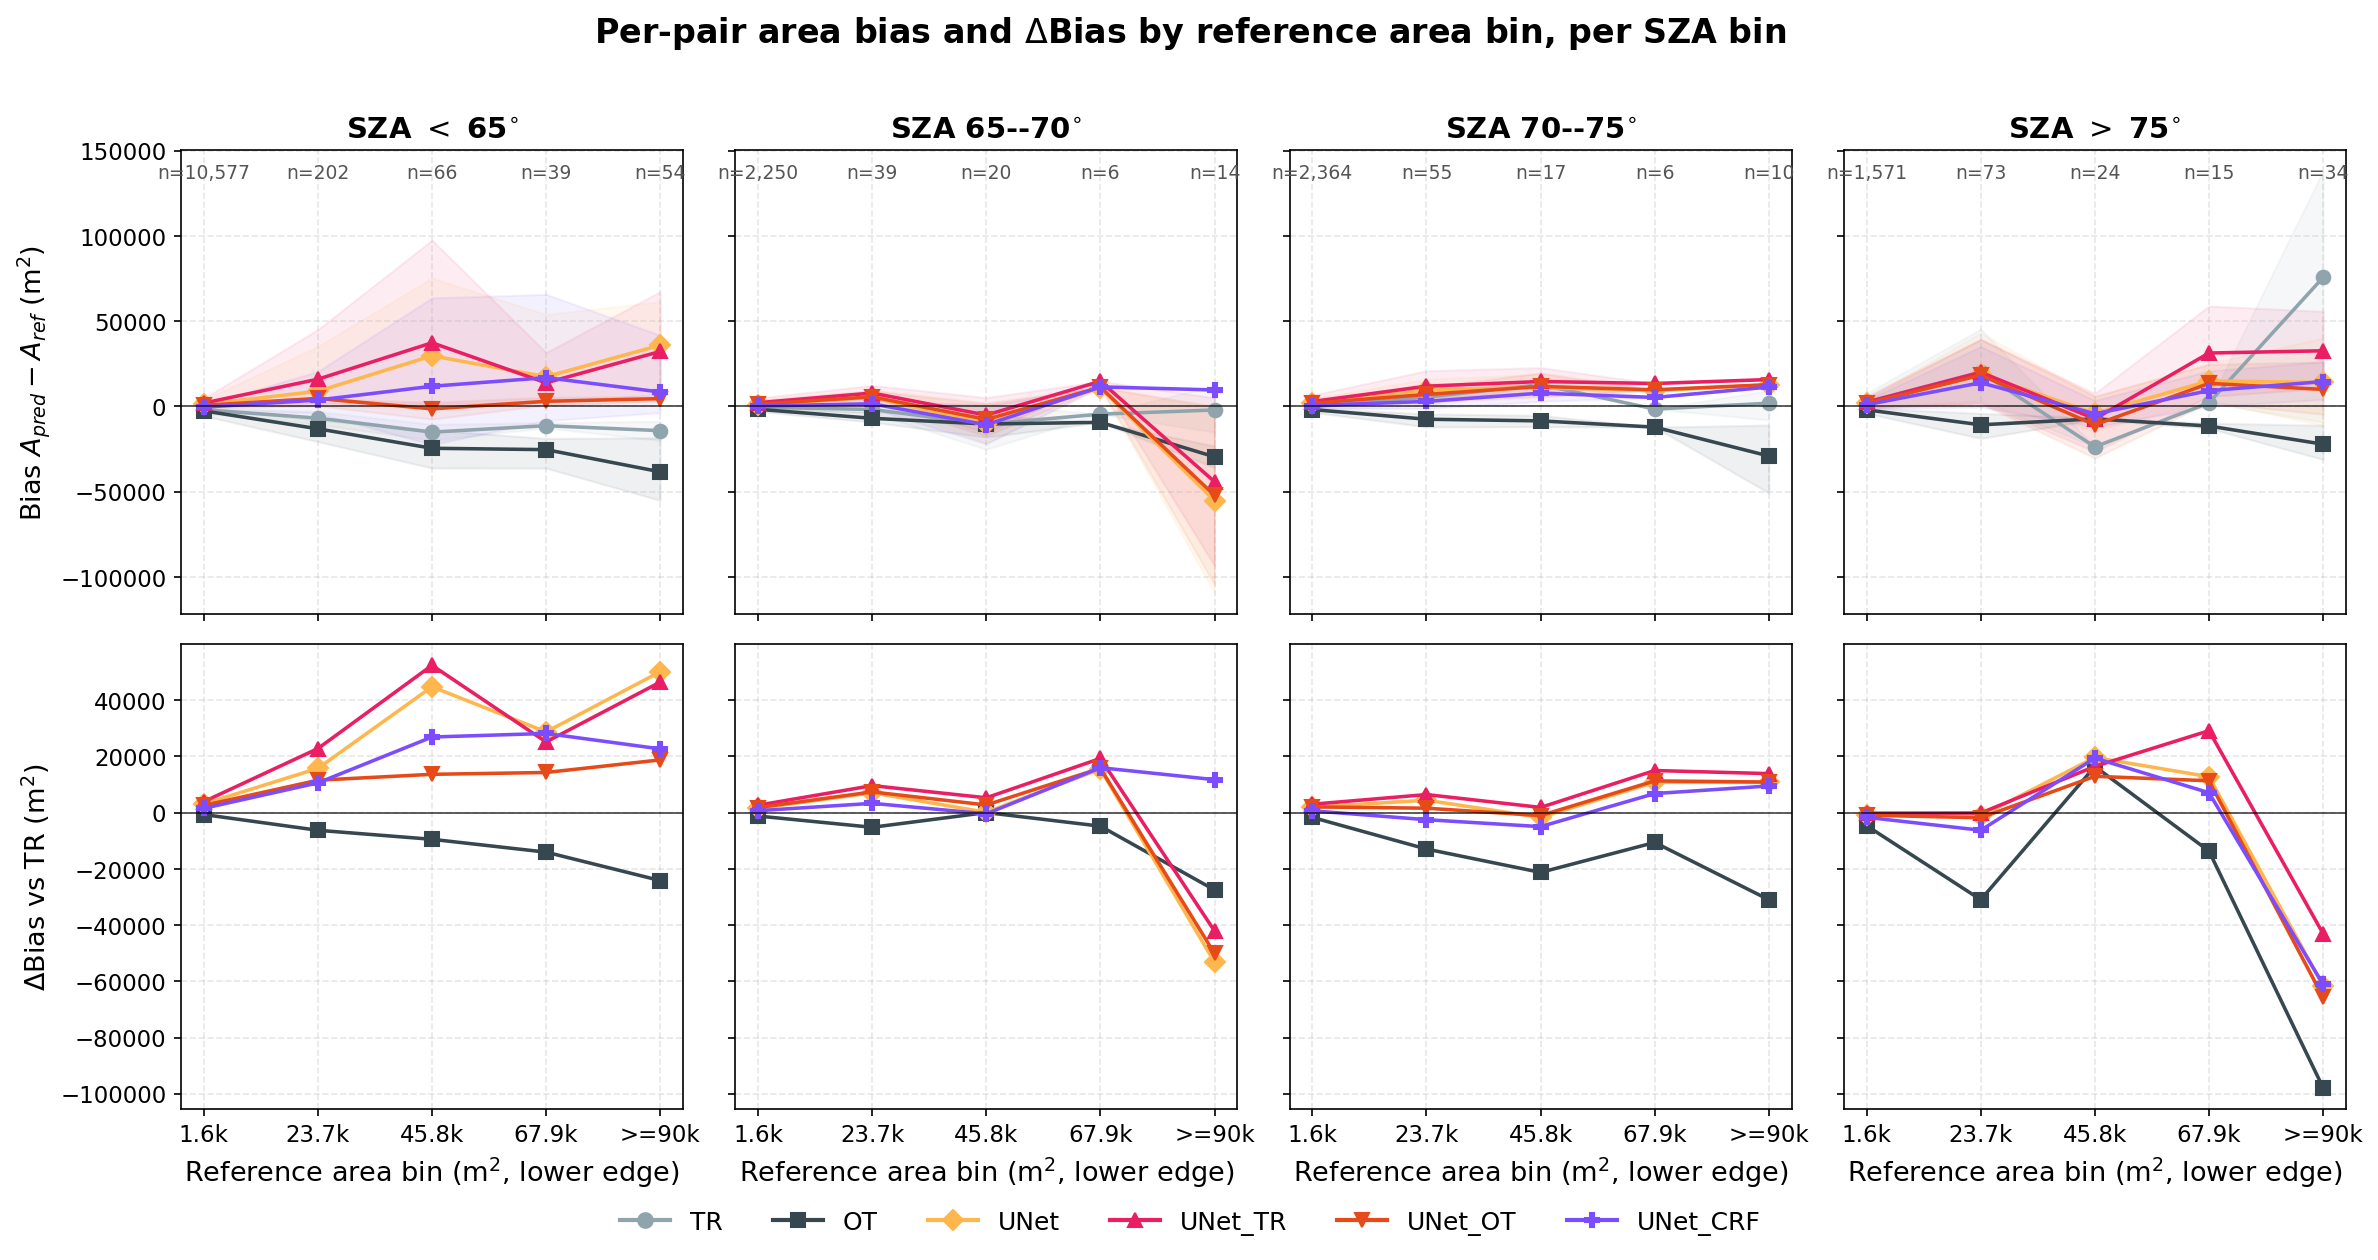
\includegraphics[width=0.95\linewidth]{figures/fig-archive/20260505_152451__bias_delta_by_area.png}
\caption{\textbf{Fig. 8.} Top row: per-pair bias (predicted minus reference iceberg area) by reference area bin and method, one panel per SZA bin (mirroring Fig.~\ref{fig:area_scatter} and Fig.~\ref{fig:re_by_area_bin}), with the P10--P90 band shaded. Bottom row: $\Delta$bias relative to the TR threshold baseline, same per-SZA panel layout. Y-axes are shared within each row so cross-SZA comparison reads off a common scale. Area bin edges (1.6k, 23.7k, 45.8k, 67.9k, 90k m$^2$) match Fisser (2025) Fig. 16. Color palette matches Fig.~\ref{fig:area_scatter} (UNet\_TR pink). Per-(SZA, area-bin) total n\textsubscript{pairs} annotated near the top of each bias panel.}
\label{fig:bias_delta_by_area}
\end{figure}

\begin{figure}[h]
\centering
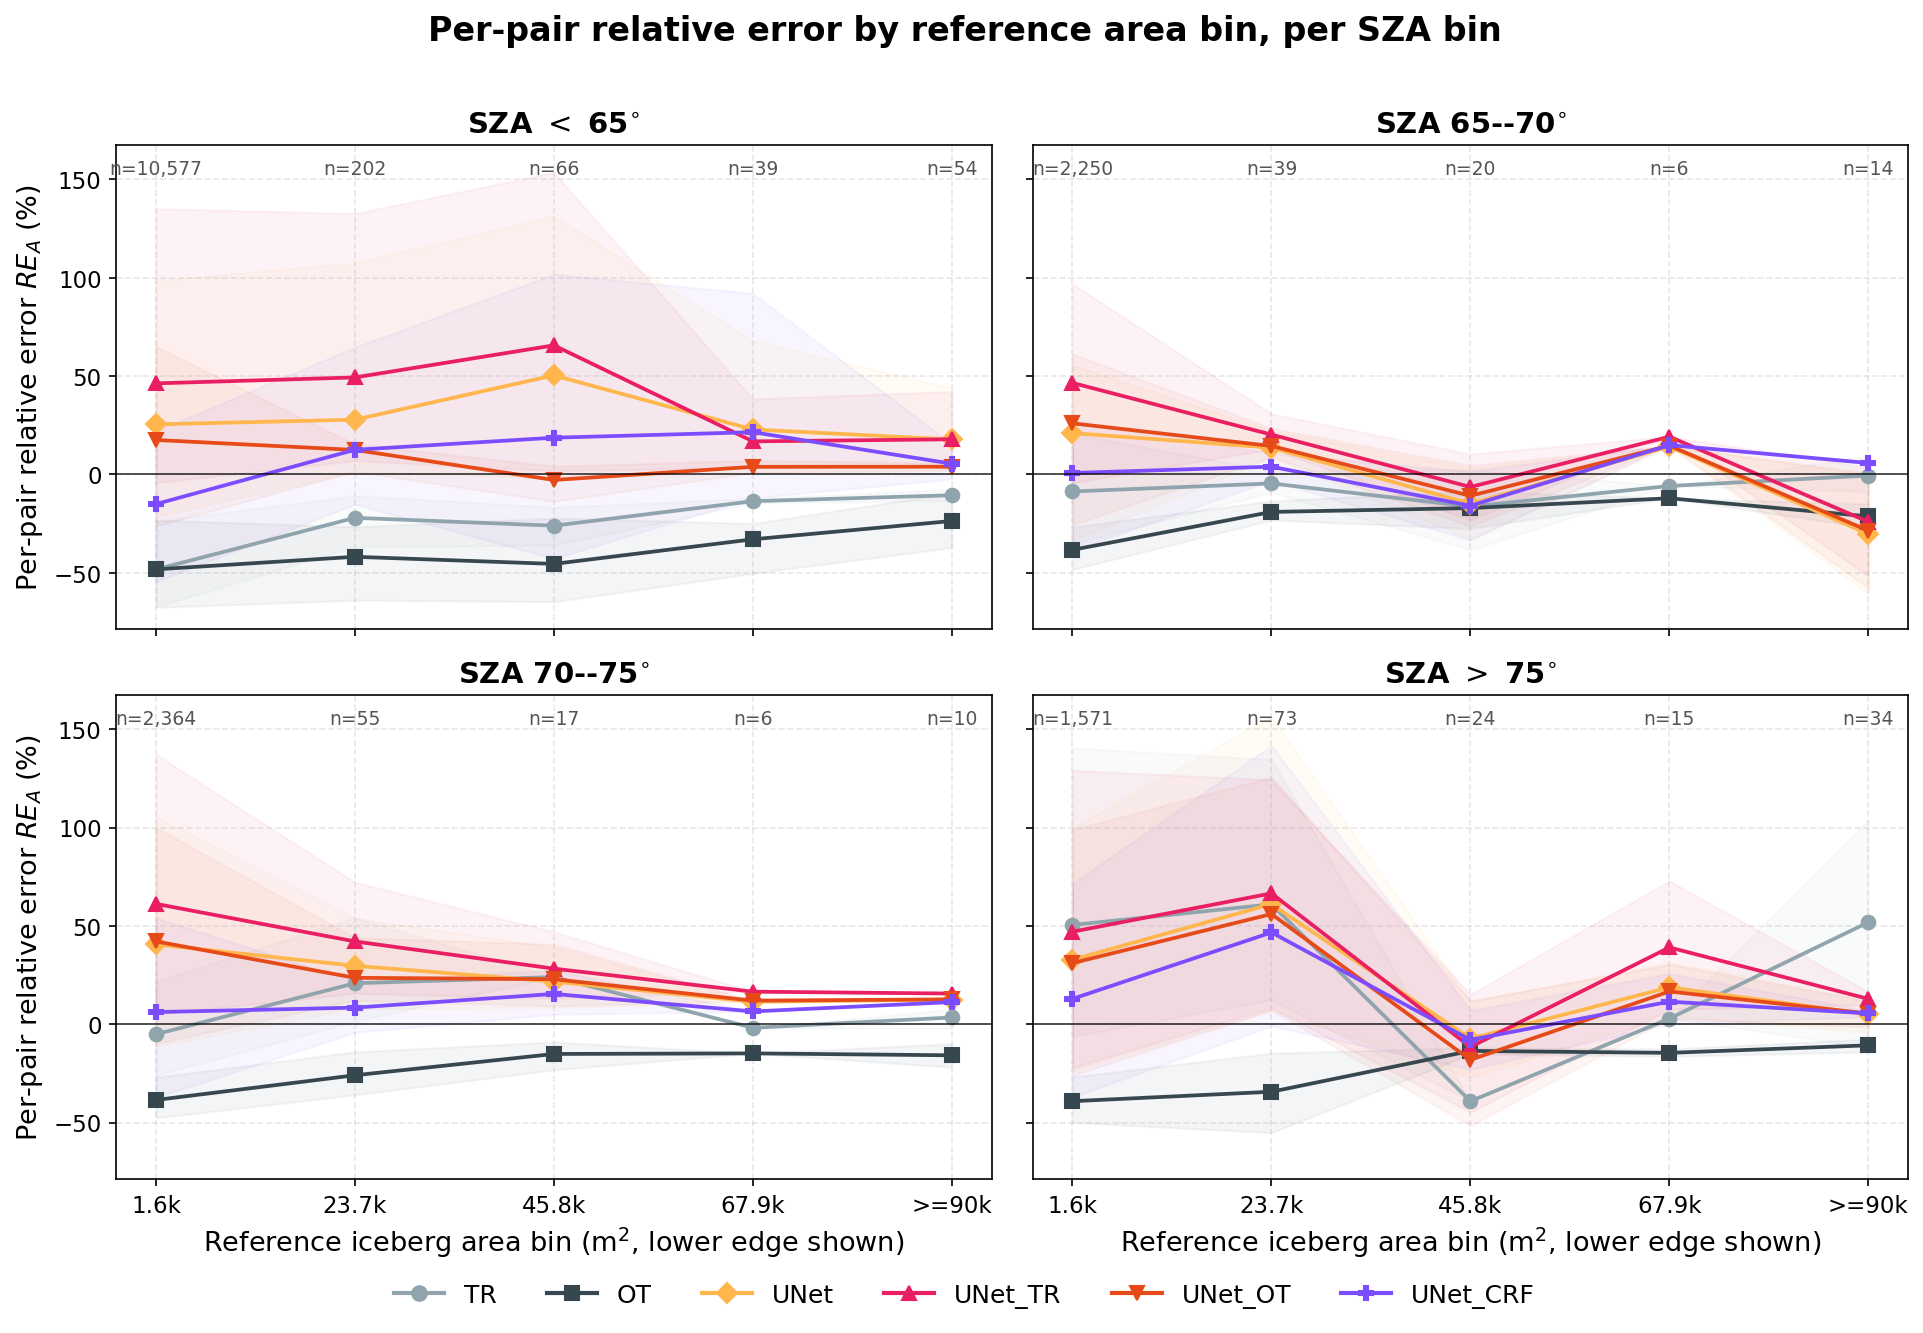
\includegraphics[width=0.95\linewidth]{figures/fig-archive/20260505_152454__re_by_area_bin.png}
\caption{\textbf{Fig. 9.} Per-pair relative error in iceberg area as a function of reference area bin, one panel per SZA bin (mirroring Fig.~\ref{fig:area_scatter}) and one line per method. Faint shaded band shows the P10--P90 spread per method per bin; mean is the solid line. Per-(SZA, area-bin) total matched-pair counts are annotated near the top of each panel. Area bin edges match Fisser (2025) Fig. 12 / 16; method palette matches Fig.~\ref{fig:area_scatter} (UNet\_TR pink). Fisser (2024) Fig. 7 / Fisser (2025) Fig. 12 analog.}
\label{fig:re_by_area_bin}
\end{figure}

\begin{table}[h]
\caption{\textbf{Table 3.} Detection statistics on the v4\_clean test split. \textit{n}\textsubscript{matched} is the count of pred--ref pairs surviving the IoU $\geq$ 0.30 filter; precision = \textit{n}\textsubscript{matched} / \textit{n}\textsubscript{pred}.}
\centering
\begin{tabular}{lrrrrr}
\toprule
Method & \textit{n}\textsubscript{ref} & \textit{n}\textsubscript{pred} & \textit{n}\textsubscript{matched} & Match rate (\%) & Precision (\%) \\
\midrule
TR        & 7201 & 16975 & 1465 & 20.3 & 8.6 \\
OT        & 7201 & 42429 & 2472 & 34.3 & 5.8 \\
UNet      & 7201 & 10878 & 3927 & 54.5 & 36.1 \\
UNet\_TR  & 7201 & 11196 & 3503 & 48.7 & 31.3 \\
UNet\_OT  & 7201 & 5702  & 1906 & 26.5 & 33.4 \\
UNet\_CRF & 7201 & 13031 & 4163 & \textbf{57.8} & 32.0 \\
\bottomrule
\end{tabular}
\end{table}

\subsection{Preprocessing pipeline as a controlled variable}

The 40 m root-length filter and the annotation-aware ice-coverage mask are applied to all training, validation, and test chips in v4\_clean. Both operations are part of our pipeline and are absent from the original Fisser data preparation. Auditing the lt65 split of v4\_clean against the raw Fisser pkls quantifies their footprint: the 40 m filter removes 41,644 of 70,818 mask components (58.8\%) and alters 312 of 330 chips; the IC mask zeros pixels in 129 of 226 training chips (57.1\%). Because both interventions substantially edit the data, the design treats preprocessing as a controlled variable rather than a fixed setting.

Table 4 reports the same headline metrics as Table 1 on the v4\_raw test split, which matches v4\_clean's split policy (65/15/25 stratified, seed 42) but disables both preprocessing operations across all chips and all bins. The training chip count is 592 (vs. 551 in v4\_clean) because no chips are dropped by the IC chip-drop. The delta between Tables 1 and 4 attributes performance differences to the preprocessing pipeline alone, integrated over the same dataset family.

\begin{table}[h]
\caption{\textbf{Table 4.} Per-pair MAE of iceberg root length (m) on the v4\_raw test split (no 40 m filter, no IC mask, all 984 chips, same split seed as v4\_clean). Lower is better.}
\centering
\begin{tabular}{lrrrr}
\toprule
Method & $<$ 65$^\circ$ & 65--70$^\circ$ & 70--75$^\circ$ & $>$ 75$^\circ$ \\
\midrule
TR        & 17.0           & 6.9            & 5.8            & 11.2 \\
OT        & 15.6           & 12.8           & 13.0           & 13.3 \\
UNet      & 9.5            & 10.7           & 10.7           & 8.7  \\
UNet\_TR  & 12.3           & 16.0           & 17.1           & 12.0 \\
UNet\_OT  & 8.2            & 11.7           & 11.1           & 9.6  \\
UNet\_CRF & 9.7            & 6.6            & 7.3            & 11.7 \\
\bottomrule
\end{tabular}
\end{table}

The dominant pattern in Tables 1 vs 4 is at the high-SZA end: every method reports a lower MAE on v4\_raw at SZA $>$ 75$^\circ$ (12.6--20.1 m on v4\_clean drops to 8.7--13.3 m on v4\_raw), and per-pair counts (\textit{n}\textsubscript{pairs}) approximately quadruple. Both effects trace to the 40 m filter: when small components are retained, the test chip's reference count is higher, and the matched pairs include short icebergs whose absolute errors are bounded by the chip resolution (10 m). The lt65 row tells the same story at smaller magnitude: UNet's MAE drops from 10.5 m to 9.5 m, with 6,769 matched pairs on v4\_raw versus 2,814 on v4\_clean.

Table 5 reports per-pair mean IoU on v4\_raw, the companion to Table 2. The IoU column moves in the opposite direction from MAE: every method's IoU is lower on v4\_raw than on v4\_clean (UNet at lt65 drops from 0.70 to 0.62; UNet\_OT at lt65 from 0.73 to 0.63). Cleaner ground truth (40 m filter applied, mask boundaries pruned) raises IoU because predicted polygons overlap a smaller, more conservative reference set. Reporting MAE and IoU in parallel is necessary; reporting either alone would obscure half the preprocessing effect.

\begin{table}[h]
\caption{\textbf{Table 5.} Per-pair mean IoU on matched iceberg pairs, v4\_raw test split. Higher is better. Bold marks the best method per SZA bin.}
\centering
\begin{tabular}{lrrrr}
\toprule
Method & $<$ 65$^\circ$ & 65--70$^\circ$ & 70--75$^\circ$ & $>$ 75$^\circ$ \\
\midrule
TR        & 0.43           & 0.60           & \textbf{0.61}  & 0.56 \\
OT        & 0.47           & 0.53           & 0.53           & 0.53 \\
UNet      & 0.62           & 0.62           & 0.60           & \textbf{0.60} \\
UNet\_TR  & 0.59           & 0.57           & 0.55           & 0.58 \\
UNet\_OT  & \textbf{0.63}  & 0.61           & 0.61           & 0.59 \\
UNet\_CRF & 0.55           & \textbf{0.63}  & 0.60           & 0.58 \\
\bottomrule
\end{tabular}
\end{table}

Table 6 isolates the preprocessing pipeline at fixed dataset scope (lt65 only, single training run per cell). A0 trains on the 398 lt65 Fisser chips with their original masks; A2 trains on the 330 chips that survive our IC chip-drop with the 40 m and IC interventions applied. Both experiments use the same UNet++ architecture, the same seed, and identical inference pipelines. Per-pair MAE is consistently higher under A2 across all six methods; per-pair IoU is mixed (TR and OT improve marginally, UNet variants worsen). Detection precision collapses for the UNet variants under A2 (UNet 6.6\%, UNet\_TR 0.04\%, UNet\_OT 4.8\%, UNet\_CRF 10.2\%) versus A0 (33--58\%). The full Phase A progression (Table 7) confirms the A0 to A2 cell as the dominant Phase A delta and shows that downstream balancing schemes do not recover the lost calibration.

\begin{table}[h]
\caption{\textbf{Table 6.} Preprocessing-pipeline isolation on lt65. A0 = Fisser preprocessing (no 40 m, no IC mask, 398 chips). A2 = our preprocessing (40 m + IC mask, 330 chips). Both train one UNet++ from scratch on the same seed. Lower MAE is better; higher IoU is better.}
\centering
\begin{tabular}{l rr rr rr}
\toprule
       & \multicolumn{2}{c}{MAE\textsubscript{RL} (m)} & \multicolumn{2}{c}{Mean IoU} & \multicolumn{2}{c}{Precision (\%)} \\
\cmidrule(lr){2-3} \cmidrule(lr){4-5} \cmidrule(lr){6-7}
Method & A0 & A2 & A0 & A2 & A0 & A2 \\
\midrule
TR        & 17.0 & 17.8 & 0.44 & 0.48 & 25.5 & 13.8 \\
OT        & 16.4 & 23.0 & 0.46 & 0.47 & 17.3 &  9.4 \\
UNet      &  9.8 & 15.3 & 0.63 & 0.47 & 58.4 &  6.6 \\
UNet\_TR  & 12.3 & 11.4 & 0.59 & 0.40 & 50.5 &  0.04 \\
UNet\_OT  &  8.2 & 33.1 & 0.64 & 0.45 & 56.1 &  4.8 \\
UNet\_CRF & 11.0 & 25.8 & 0.56 & 0.51 & 44.3 & 10.2 \\
\bottomrule
\end{tabular}
\end{table}

\subsection{Phase A leaderboard and calibration mechanism}

Phase A walks four controlled variables on lt65-only chips: preprocessing pipeline (A0 to A2), null-chip injection (A0 to A1, A2 to A3), augmentation (A3 to A4), and class plus size balancing (A4 to A9). All ten experiments use byte-identical hyperparameters (ResNet34 encoder, 100 epochs, learning rate 1 $\times$ 10$^{-4}$, batch size 16, seed 42); only the training data and the balancing scheme differ. Table 7 reports best validation IoU and test IoU on the lt65 split, ordered by best validation IoU.

\begin{table}[h]
\caption{\textbf{Table 7.} Phase A leaderboard. UNet match rate is the per-pair detection rate at IoU $\geq$ 0.30; UNet RL MAE is the per-pair mean absolute error in iceberg root length on matched pairs. All columns evaluated on the lt65 test split.}
\centering
\begin{tabular}{llrrrr}
\toprule
ID & Manifest & val IoU & test IoU & UNet match rate & UNet RL MAE (m) \\
\midrule
A0 & v4\_raw\_lt65 (Fisser preprocessing, no nulls)            & \textbf{0.613} & \textbf{0.577} & \textbf{0.512} & \textbf{9.82} \\
A1 & v4\_raw\_lt65\_plus\_nulls (Fisser preprocessing + nulls) & 0.503 & 0.477 & 0.315 & 15.21 \\
A3 & v4\_clean\_lt65\_plus\_nulls                              & 0.269 & 0.336 & 0.182 & 15.69 \\
A2 & v4\_clean\_lt65 (our preprocessing, no nulls)             & 0.261 & 0.344 & 0.245 & 15.26 \\
A7--A9 & v4\_clean + nulls + aug + size oversample             & 0.243 & 0.320 & 0.163 & 14.78 \\
A5--A6 & v4\_clean + nulls + aug + class balance               & 0.237 & 0.312 & 0.158 & 15.23 \\
A4 & v4\_clean + nulls + aug                                   & 0.225 & 0.274 & 0.122 & 14.93 \\
\bottomrule
\end{tabular}
\end{table}

A0 wins on every metric. The gap to A1 (0.11 IoU) measures the cost of null-chip injection at a 1:1 GT$+$ : GT0 ratio under Fisser preprocessing. The gap to A2 (0.35 IoU) measures the cost of our preprocessing pipeline alone. Once preprocessing is applied, no balancing scheme moves the result by more than 0.05 IoU.

The grouped rows in Table 7 reflect an empirical collapse of the planned 2x3 balancing grid. A5 and A6 produce identical training sets (87 chips) because the v4\_clean\_lt65\_plus\_nulls manifest's GT$+$ class is the natural majority (198 vs. 29, ratio 6.8:1), so the adaptive scheme resolves to the same direction as the fixed-positive scheme. A7, A8, and A9 also produce identical training sets (110 chips) because the size-oversample step bottoms out at the same equilibrium under the 4x replication cap regardless of upstream class balancing. The grid reduces empirically to three distinct training conditions (A4 at 58 chips, A5 / A6 at 87, A7 / A8 / A9 at 110), all within 0.02 best validation IoU of each other.

To probe the mechanism behind the A0 to A2 collapse, we sampled ten lt65 prob-tifs from each run and computed the median pixel value of the UNet++ softmax P(iceberg) band (Table 8). Baseline\_v1 and A0 produce sharply bimodal distributions: most pixels collapse near zero, only confident iceberg pixels rise above 0.5. A2's distribution is diffuse, with the majority of pixels in the 0.20--0.35 range that any fixed threshold below 0.35 misclassifies as iceberg. The downstream consequence is visible in UNet\_TR predicted polygons: median area is 2,200 m$^2$ on baseline\_v1, 1,600 m$^2$ on A0, and 200 m$^2$ on A2; 49 \% of A2's predicted polygons fall below 200 m$^2$, all speckle.

\begin{table}[h]
\caption{\textbf{Table 8.} P(iceberg) distribution on the lt65 test split, median across ten sample chips per run. The 0.20--0.35 column is the threshold-relevant range any fixed-threshold method below 0.35 will sweep into the iceberg class.}
\centering
\begin{tabular}{lrrr}
\toprule
Run & median P(iceberg) & frac. pixels 0.20--0.35 & frac. pixels $\geq$ 0.5 \\
\midrule
baseline\_v1   & 0.001 & 0.4 \%  & 4.0 \% \\
A0 (raw lt65)  & 0.013 & 2.2 \%  & 6.6 \% \\
A2 (clean lt65) & 0.278 & \textbf{59.0} \% & 5.2 \% \\
\bottomrule
\end{tabular}
\end{table}

The calibration shift is a property of the data, not the code. The IC pixel mask zeros bright non-annotated pixels in 112 of A2's 198 training chips (57 \%); the validation and test splits are never masked. The model trains on partially zeroed images and encounters fully bright pixels at inference, producing the diffuse predictions visible in Table 8. Applying Fisser's preprocessing pipeline in a low-data, lt65-only regime degrades model calibration to the point that no fixed-threshold post-processing recovers it. Fig.~\ref{fig:outline_examples} illustrates the qualitative effect of these calibration choices on the canonical baseline, showing reference and UNet\_CRF predicted iceberg outlines on representative chips per SZA bin.

\begin{figure}[h]
\centering
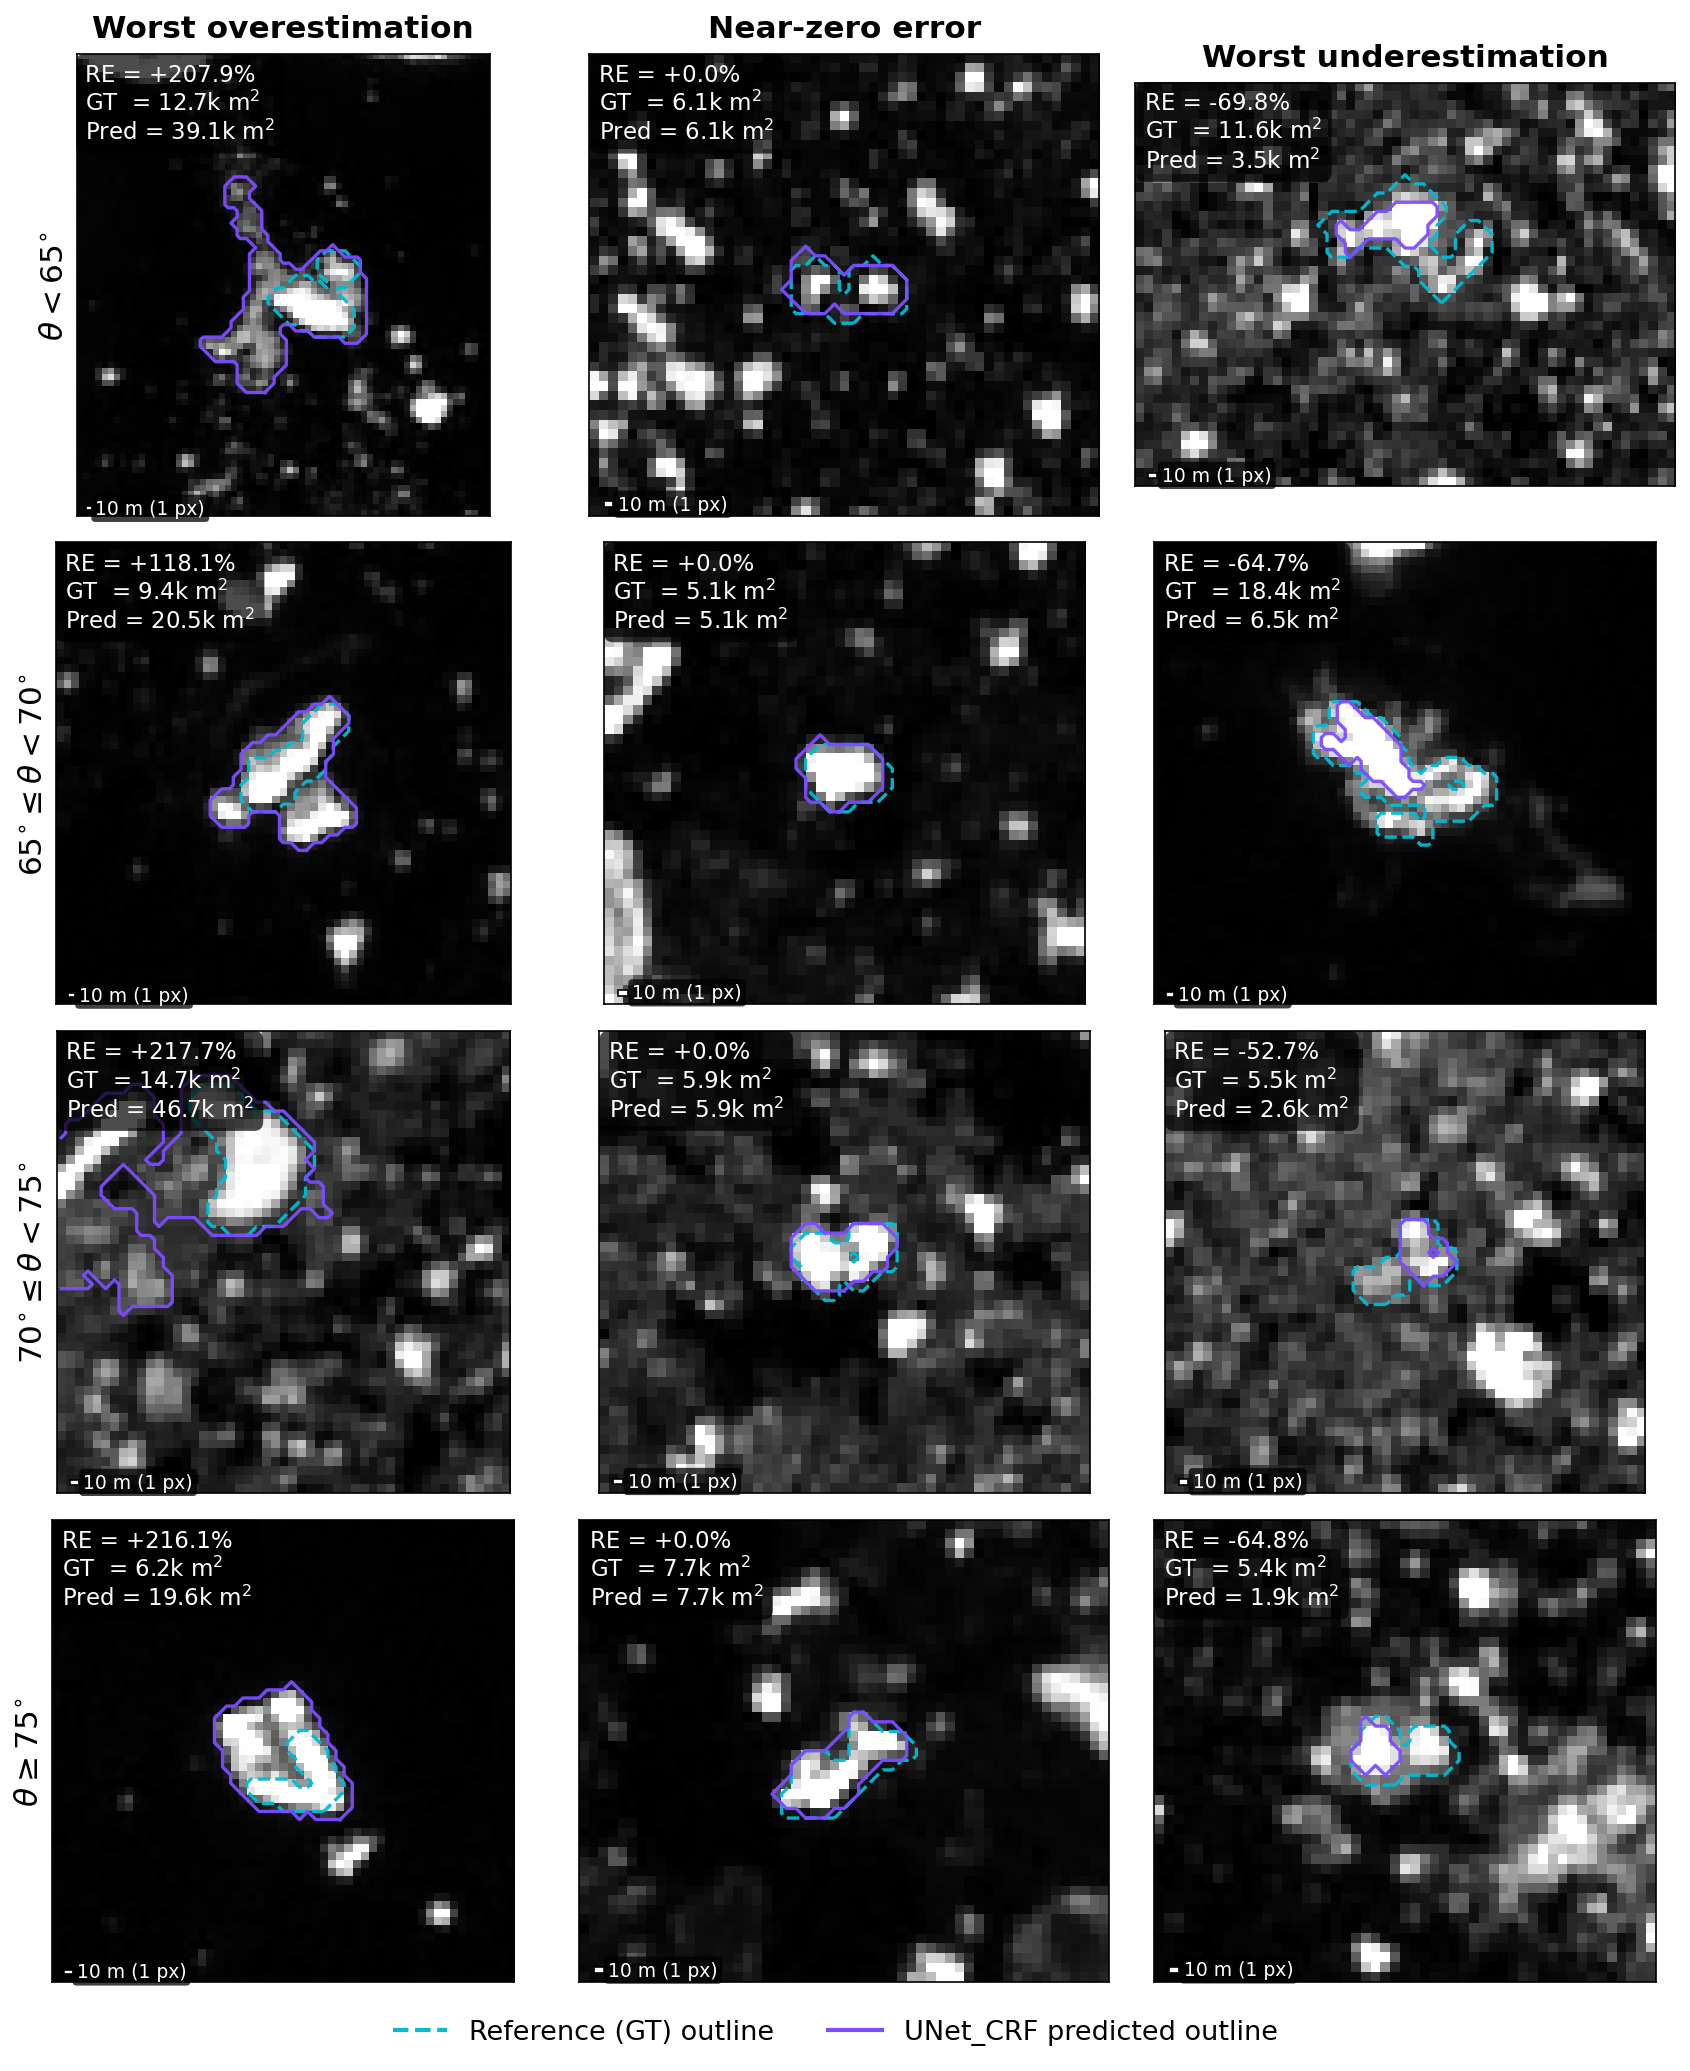
\includegraphics[width=0.95\linewidth]{figures/fig-archive/20260505_152459__outline_examples.png}
\caption{\textbf{Fig. 10.} Per-SZA-bin chip examples with reference (cyan dashed) and UNet\_CRF predicted (bright purple solid; same color as UNet\_CRF in Figs.~\ref{fig:area_scatter}--\ref{fig:re_by_area_bin}) iceberg outlines, picked at three per-pair RE positions: worst-positive, near-zero, worst-negative (chips with reference area below 5{,}000 m$^2$ excluded). B08 NIR backdrop; each panel is cropped to a 20 px context margin around the matched-pair iceberg bbox so the outlines have visual breathing room and are not clipped at panel edges. A 10 m scale bar (1 Sentinel-2 pixel) is drawn at the bottom-left of each panel as a ground-distance reference. Only the highlighted iceberg with cyan-dashed reference outline and purple-solid UNet\_CRF outline is the example pair; other icebergs visible in the chip background are not annotated and not included in the panel's RE / area values. Fisser (2024) Fig. 13 analog.}
\label{fig:outline_examples}
\end{figure}

\subsection{Top-hat small-iceberg recovery}

White top-hat morphological filtering on the B08 band recovers small bright objects each base method missed. For each chip the top-hat response is computed with a disk structuring element of radius 10 pixels (100 m), thresholded at 0.05 reflectance units, filtered to connected components $\geq$ 16 pixels, and unioned with the base method's polygons; pixels already covered by the base method are excluded from the recovery candidate set. The same recovery step is applied uniformly to all six base methods, producing six $+$TH variants. Tables 9 and 10 report per-pair MAE on root length and per-pair mean IoU after recovery; Table 11 reports detection statistics.

\begin{table}[h]
\caption{\textbf{Table 9.} Per-pair mean absolute error of iceberg root length (m) on the v4\_clean test split after top-hat recovery. Lower is better. Bold marks the best method per SZA bin.}
\centering
\begin{tabular}{lrrrr}
\toprule
Method & $<$ 65$^\circ$ & 65--70$^\circ$ & 70--75$^\circ$ & $>$ 75$^\circ$ \\
\midrule
TR$+$TH        & 17.1           & \textbf{8.0}   & \textbf{11.0}  & 20.4 \\
OT$+$TH        & 17.4           & 12.6           & 13.8           & \textbf{19.5} \\
UNet$+$TH      & 10.3           & 12.0           & 17.5           & 23.2 \\
UNet\_TR$+$TH  & 13.9           & 15.8           & 20.4           & 24.4 \\
UNet\_OT$+$TH  & 13.2           & 12.5           & 16.4           & 22.0 \\
UNet\_CRF$+$TH & \textbf{10.0}  & 8.5            & 12.9           & 20.7 \\
\bottomrule
\end{tabular}
\end{table}

\begin{table}[h]
\caption{\textbf{Table 10.} Per-pair mean IoU on matched iceberg pairs after top-hat recovery. Higher is better.}
\centering
\begin{tabular}{lrrrr}
\toprule
Method & $<$ 65$^\circ$ & 65--70$^\circ$ & 70--75$^\circ$ & $>$ 75$^\circ$ \\
\midrule
TR$+$TH        & 0.51           & 0.66           & \textbf{0.65}  & 0.60 \\
OT$+$TH        & 0.52           & 0.61           & 0.62           & 0.58 \\
UNet$+$TH      & \textbf{0.72}  & 0.66           & 0.64           & \textbf{0.60} \\
UNet\_TR$+$TH  & 0.68           & 0.64           & 0.61           & 0.59 \\
UNet\_OT$+$TH  & 0.62           & 0.66           & 0.64           & 0.60 \\
UNet\_CRF$+$TH & 0.67           & \textbf{0.68}  & \textbf{0.66}  & \textbf{0.61} \\
\bottomrule
\end{tabular}
\end{table}

\begin{table}[h]
\caption{\textbf{Table 11.} Detection statistics after top-hat recovery. Match rate rises uniformly relative to Table 3 because the recovered components contribute additional matched pairs at small root length; precision drops because TH adds polygons that are sometimes spurious bright objects.}
\centering
\begin{tabular}{lrrrrr}
\toprule
Method & \textit{n}\textsubscript{ref} & \textit{n}\textsubscript{pred} & \textit{n}\textsubscript{matched} & Match rate (\%) & Precision (\%) \\
\midrule
TR$+$TH        & 7201 & 28342 & 2851 & 39.6 & 10.1 \\
OT$+$TH        & 7201 & 42859 & 2883 & 40.0 &  6.7 \\
UNet$+$TH      & 7201 & 14174 & 3147 & 43.7 & 22.2 \\
UNet\_TR$+$TH  & 7201 & 14080 & 2874 & 39.9 & 20.4 \\
UNet\_OT$+$TH  & 7201 & 17630 & 2963 & 41.2 & 16.8 \\
UNet\_CRF$+$TH & 7201 & 16065 & 3330 & \textbf{46.2} & 20.7 \\
\bottomrule
\end{tabular}
\end{table}

The recovery step trades precision for recall: every method's match rate rises (UNet\_CRF$+$TH 46.2 \% vs UNet\_CRF 57.8 \% in Table 3 has fewer overall predicted polygons, but TH adds more recovered candidates per chip). Per-pair IoU on lt65 stays statistically indistinguishable from the no-TH baseline for all UNet variants and improves for the threshold-only methods (TR 0.48 $\rightarrow$ 0.51, OT 0.47 $\rightarrow$ 0.52). At higher SZA bins TH is mildly counterproductive (sza\_gt75 MAE\_RL of 12.6 m for UNet\_CRF degrades to 20.7 m after TH), suggesting that the dim-illumination top-hat response under-thresholds and adds many small false positives. Reporting both tables in parallel makes the recall-precision trade-off visible per SZA bin.

\subsection{Comparison with Fisser (2024, 2025)}
% TODO: reconcile against Fisser (2024)'s +5.9% to -5.7% standardised-error band up to SZA 65 deg,
% and against Fisser (2025) dataset reference statistics in
% ../../reference/descriptive_stats_results_discussion.md §6.


\section{Discussion}

\subsection{SZA-dependent contrast compression}
% TODO. B08 reflectance facts from ../../reference/b08_analysis_results_discussion.md §1-2:
%   sza_65_70 is the worst bin for threshold methods: iceberg B08 compresses to 0.336,
%     ocean B08 is 0.160, contrast drops to 0.176 (23% below the next bin).
%   sza_gt75: iceberg mean 0.677 but bimodal; 16.5% of iceberg pixels still fall below 0.22,
%     driving shadow-based underestimation despite high mean reflectance.

\subsection{Learned segmentation robustness}
% TODO once results populate. Expected framing: spatial context lets UNet++ carry shadow-face
% pixels as iceberg because their neighbours are iceberg, avoiding the per-pixel failure mode.

\subsection{Operational implications}
% TODO: extending automated iceberg monitoring into the autumn low-illumination window.
% ESA recommends SZA <= 70 deg for Sentinel-2 acquisitions; this work tests beyond that limit.

\subsection{Limitations}
% TODO:
%   - No independent ground-truth area. Method-consistency framing, not absolute validation.
%   - Temperature confound at sza_gt75: 98.9% of chips at temp <= 0 deg C
%     (../../reference/descriptive_stats_results_discussion.md §4). Cannot disentangle SZA
%     optical effects from temperature thermal effects.
%   - Annotation-source asymmetry: Fisser 2025 chips (sza_lt65) are iceberg-rich by selection
%     (99.2% chips contain icebergs). Roboflow chips at higher SZA have ~50% null chips.
%   - 92 annotations exceed Fisser (2025) maximum area (400,000 m^2); likely multi-iceberg clumps
%     pending review (../../plan.md §Open Questions).


\section{Conclusion}
% TODO: one paragraph summarising headline findings and operational implication.


\section{Acknowledgements}
% TODO: supervisors, Fisser et al. for shared data, Bowdoin HPC, Roboflow annotators.


% JGlac bibliography: igs.bst style. igs.cls loads natbib automatically,
% so \citet{} and \citep{} are available.
\bibliography{references}
\bibliographystyle{igs}


\end{document}
